\documentclass[12pt,a4paper]{article}

\usepackage[margin=1in]{geometry}
\usepackage[english]{babel}
\usepackage[T1]{fontenc}
\usepackage[utf8]{inputenc}

\usepackage{colortbl}
\usepackage{longtable}
\usepackage{tabularx}
\usepackage{booktabs}
\usepackage{array}
\usepackage{multirow}
\usepackage{graphicx}
\usepackage{xcolor}
\usepackage{enumitem}
\usepackage[parfill]{parskip}
\usepackage[title,titletoc]{appendix}
\usepackage{amsmath}
\usepackage{fnpos}
\usepackage{geometry}
\usepackage{csquotes}
\usepackage{tikz}
\usepackage{pdflscape}

% \graphicspath{{../DOC/SLIDES/IMAGES/}}

\usetikzlibrary{positioning}
\usetikzlibrary{calc}
\tikzstyle{main} = [rectangle, rounded corners, minimum height=0.7cm,text centered, draw=black, font=\scriptsize]
\tikzstyle{process} = [rectangle, minimum height=0.7cm, text centered, draw=black, font=\scriptsize]
\tikzstyle{note} = [rectangle, text centered, minimum height=1cm]
\tikzstyle{arrow} = [->,>=stealth,auto,font=\scriptsize,node distance=3cm, main node/.style={circle,draw}]

\usepackage[hyphens]{url}

\usepackage[backend=biber,url=false,style=authoryear,sorting=nyt,bibstyle=numeric]{biblatex}
\addbibresource{chequeBounce.bib}

\usepackage[acronym,nonumberlist,nomain]{glossaries}
\newglossaryentry{adr}{name={ADR},description={Alternative Dispute Resolution}}
\newglossaryentry{crpc}{name={CrPC},description={Code of Criminal Procedure}}
\newacronym{coe}{CoE}{Committee of Experts}
\newacronym{lci}{LCI}{Law Commission of India}
\newacronym{ni}{NI Act}{Negotiable Instruments Act, 1881}
\newacronym{njdg}{NJDG}{National Judicial Data Grid}
\newacronym{sci}{SCI}{Supreme Court of India}
\newacronym{ut}{UT}{Union Territory}

\AtBeginEnvironment{quote}{\smaller}
\makeFNbottom
\geometry{margin=1in}
\renewcommand{\baselinestretch}{1.25}
\setlength{\parskip}{1em}
\setlist{nosep}

\newcommand{\floattabu}[1]{
\vspace*{0.2in}
{\footnotesize
#1
}
\vspace*{0.2in}}

\usepackage[hidelinks,breaklinks,colorlinks=true,allcolors=blue,citecolor = blue]{hyperref}
\usepackage{cleveref}

\title{Characterising cheque dishonour cases in India: Causes for delays and policy implications}
\author{Devendra Damle\thanks{Devendra Damle is a researcher at the National Institute of Public Finance and Policy.} \and Jitender Madaan\thanks{Jitender Madaan is an Associate Professor at the Indian Institute of Technology, Delhi.} \and Karan Gulati\thanks{Karan Gulati is a researcher at the Vidhi Centre for Legal Policy.} \and Manish Kumar Singh\thanks{Manish Kumar Singh is an Assistant Professor at the Indian Institute of Technology, Roorkee.} \and Nikhil Borwankar\thanks{Nikhil Borwankar is a practising advocate.}}

\begin{document}
\maketitle

\begin{abstract}

This paper analyses the determinants of case disposition time under the Negotiable Instruments Act, 1881 by creating a unique dataset of roughly 50,000 case level records spread across ten major States in India. Unlike previous studies, this analysis focuses mainly on case characteristics directly linked with procedural matters to estimate the case duration. Regression results show that multiplicity of proceedings, non-appearance of accused, trials being run as summons trial, jurisdictional issues, and reference to mediation significantly increase the case duration. These findings are robust even when considering the number of hearings as a proxy for case disposition time. Additionally, results indicate that, on average, contested cases have a lower duration. However, it takes roughly three additional hearings to resolve. These estimates also indicate that the 2015 amendment to the Negotiable Instruments Act, 1881, which focused on clarifying the jurisdiction issues, and mandatory centralisation of cases against the same drawer, has reduced the case duration by six months.

\end{abstract}

\textit{Keywords: } Negotiable Instruments Act, cheque bouncing, disposition time, court delay, procedural reforms

\textit{JEL Classification:} K12, K19, K41

\newpage
\tableofcontents

\newpage
\section{Introduction}
\label{sec:introduction}

India has a slow judiciary --- courts are clogged with large backlogs \autocite{moog1992delays, debroy2008justice, dutta2019modernise}. As of 8th December 2021, over forty-one million cases were pending across district courts \autocite{njdg2021}. It is estimated that judicial delays cost India around 1.5\% of its GDP annually \autocite{dey2016_cost}. Slow judiciaries also have adverse consequences on the structure and efficiency of markets and the quality of life of citizens \autocite{world2004world, chemin2007impact, rao2020institutional}. Therefore, it is hardly surprising that tackling judicial delay has become a top priority for Indian judges and policymakers.

One reason for the large burden on courts is believed to be the large share of \gls{ni} cases.\footnote{In particular, \S~138 of the Negotiable Instruments Act (Dishonour of a cheque for insufficiency, etc., of funds in the account). Act 26 of 1881} While the NI Act contains several provisions that may lead to a dispute, \S~138, in particular, provides that if a cheque (drawn by a person for paying off a debt or a liability) is returned unpaid due to insufficiency of funds or credit, the payer may be imprisoned for up to two years or with a fine up to twice the amount of the cheque, or both. As per the \gls{lci}, they represent 6.5\% and 7.8\% of all institutions and pendency in Indian courts, respectively \autocite{lci2014_arrears}. As per one order of the Supreme Court of India, they reflect more than 15\% of all criminal cases in the District Courts \autocite{sc2020_makwanavstate}. As per another order, they constitute over 30\% of the total pendency in courts.\footcite[Similarly, a study published by the Department of Justice briefly touches on the burden of such cases on the judiciary and posits that they constitute 34\% of pending criminal cases in Maharashtra.][]{sc2020_138, mahadik2018_maharashtra}

Given this increasing volume and persistent mention of \gls{ni} cases as a major cause of judicial delay, \textcite{sridhar2017_cheque} examined the behaviour of cheque dishonour cases in India by looking at the DAKSH database of 67,000 cases spread across Indian courts. In most cases, the authors found that resolution is delayed well beyond the statutorily prescribed timeline of 180 days. Using 50,000 case level data for eight States and two Union Territories, we also estimate the survival probability (using non-parametric Kaplan-Meier estimation) to understand the proportion of unresolved cases within the stipulated time.\footnote{The dataset used for this analysis is documented in section \ref{sec:data-description}.} Figure \ref{fig:stateSurvival} shows the survival probability (case ongoing) for the \gls{ni} cases for different States. As per our estimate, less than 20\% of the cases get disposed of within the prescribed timeline of 180 days. Also, the probability of case completion within 500 days is less than 50\% for most States.

\begin{figure}[!ht]
\centering
\caption{Survival probability of cases across States}\label{fig:stateSurvival}
\footnotesize
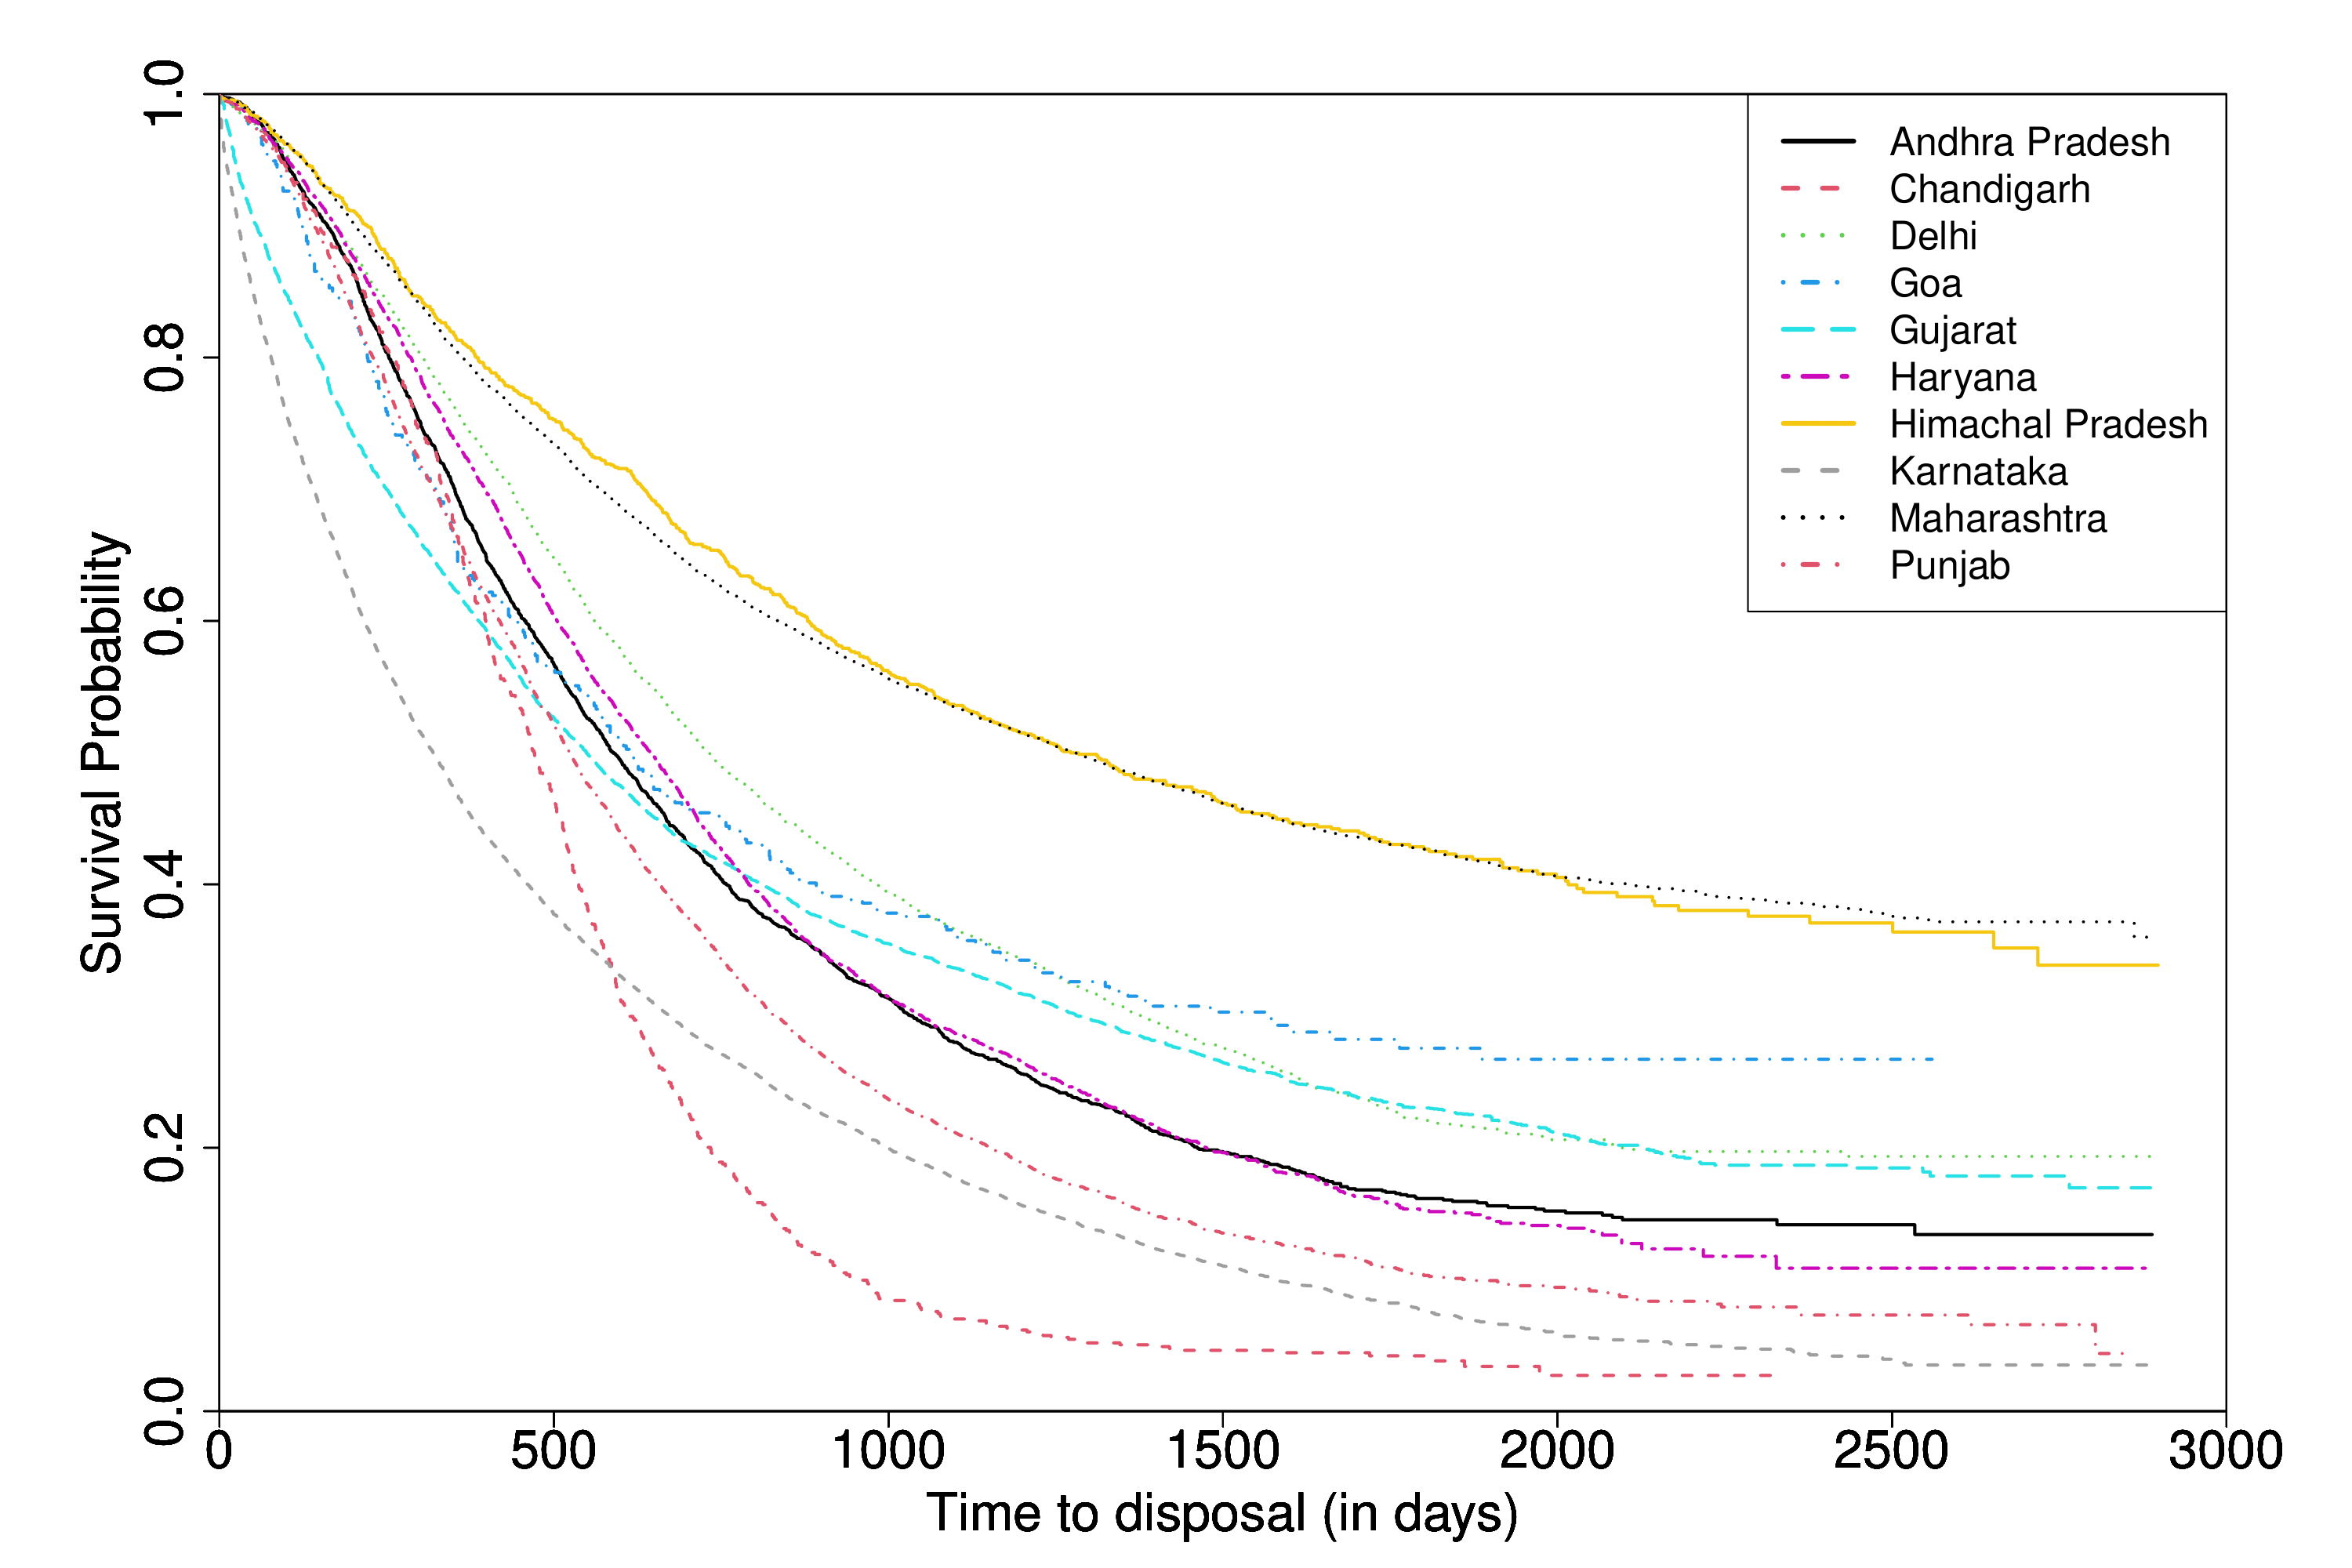
\includegraphics[width=\textwidth]{surv_states-1.png}
\textit{Note:} The X-axis shows the number of days that a case takes from the date of admission until the outcome. The Y-axis shows the probability of the case continuing up to a given number of days.
\end{figure}

Since cheque dishonour cases are a large burden on the judiciary, various committees, institutions, and government bodies have focused on expediting disposal. For example, the \textcite{lci2008_138}, by relying on newspaper reports concerning the proportion of cheque dishonour cases, recommended setting up Fast Track Magisterial Courts (for a detailed discussion, refer to \textcite{bhan2015_placing}). The Act was also subject to amendments in 2015 and 2018 to deal with the various procedural matters. Similarly, the Supreme Court has issued directions to lower courts and various financial institutions to take a more pragmatic and realistic approach for the speedy disposal of \gls{ni} cases.

In 2020, the Supreme Court of India took on board a suo-motu case concerning the “expeditious trial of cases under section 138 of the Negotiable Instruments Act 1881” \autocite{sc2020_138}. Among other directions, the court formed a \gls{coe}\footnote{Headed by Hon’ble Mr. Justice RC Chavan, former Judge of the Bombay High Court.} and appointed Amici Curiae\footnote{Mr. Sidharth Luthra (Sr Advocate) and Mr. K Parameshwar (Advocate).} to assist the court, to study processes to expedite the disposal of complaints under \S~138 of the \gls{ni}. In late 2020, the Amici submitted their recommendations. This included (i) increasing the use of pre-and post-summons mediation, (ii) expediting the service of summons to reduce absconsion, (iii) addressing the multiplicity of proceedings, etc. (for additional detail, refer to \autocite{amicus2020_submission}).

Given this background, the purpose of this paper is fourfold. First, using case level eCourts data, for the first time in India, we estimate the real judicial caseload due to the \gls{ni}. Second, we estimate the average case disposal time and its variation over time and across States. Third, we build a conceptual framework to establish the link between specific case characteristics and procedural delay. Furthermore, we empirically test our conceptual framework of procedural determinants of case disposal time using regression analysis. In line with \textcite{bielen2015}, using case level interim and final orders data, we establish the link between the specific case characteristics and procedural issues while controlling for inherent court and judge characteristics. The empirical literature on the length of court proceedings currently focuses mainly on determinants at the country and court levels, e.g. public budgets for courts, backlogs, number of judges, etc. Some studies also focus on the case level determinants like the number of parties involved, number of pleadings, etc. Given access to the interim and final orders data, we focus on the case characteristics that can be directly targeted using procedural reforms.

Additionally, we examine the role of the Negotiable Instruments (Amendment) Bill, 2015, which was passed by the Parliament in December 2015. The amendment focused on clarifying the jurisdiction-related issues for filing cases for an offence committed under \S~138 of the Negotiable Instruments Act, 1881. It also mandated the centralisation of cases against the same drawer. These reforms were specially drafted to accelerate court proceedings even though no evidence-based insight into the causes of prolonged trials was available. We analyse the effect of the 2015 amendment by comparing the duration of cases handled before and after their implementation using regression analysis. Our research makes it possible to evaluate the effectiveness of these reforms, at least for the States for which we gathered the data.

Our estimates suggest that cheque dishonour cases represent 13.2\% of courts' workload (pending and disposed) in India. This number could be underestimated because, in about 36\% of the cases in the sample, orders were either unavailable or could not be parsed. We also find significant variation in case disposal time across states. Median disposal time varies from as low as 218 days in Karnataka to as high as 547 days in Himachal Pradesh, with a median disposal time of 395 days for the dataset as a whole. We also find that only a fifth of the cases get disposed within the prescribed limit of six months.

Controlling for State and year fixed effects, our findings suggest that, all else being equal, cases where the accused fails to appear take an additional 201 days and 7 hearings to dispose of. Similarly, cases run as summons trials take 112 days and 7.4 hearings more than summary trials. Cases with jurisdictional issues take 271 days and 5.5 hearings more to dispose of than cases without these issues. Cases with a multiplicity of proceedings --- i.e. where multiple cheques are dishonoured and hence multiple, simultaneous cases are filed --- take an additional 168 days and 9.9 hearings to dispose of than those without. Contested cases take fewer days to dispose of than uncontested cases, even though they take more hearings. Our results also indicate that the 2015 amendments have significantly reduced case duration -- reducing the case duration by more than six months.

The rest of this paper is organised as follows: after this introduction, \cref{sec:history} elaborates on the history of cheque dishonour provisions in India and their relation to judicial delays. In \cref{sec:select-case-char}, based on our conversations with practising lawyers, other stakeholders, and the recommendations of the Amici Curiae and the Supreme Court, we figure out the key case characteristics linked to the procedural delay that can be directly targeted by court interventions. \Cref{sec:methodology} describes the methodology, and \cref{sec:results} presents the results thereof. In \cref{sec:2015amend}, we analyse the effectiveness of the 2015 amendments by comparing the duration of cases handled before and after the procedural reforms were implemented. Finally, \cref{sec:conclusion} concludes the paper and presents the way forward.

\section{Cheque dishonour and judicial delays} \label{sec:history}

The \acrlong{ni} was enacted to define the law relating to promissory notes, bills of exchange, and cheques. To increase the culture regarding the use of cheques and enhance the credibility of the instrument, the Act was amended in 1988.\footcite{niAmend1988} A new chapter (\S\S~138 to 142) was incorporated for penalties in the event of dishonour of cheques due to insufficient funds in the account of the drawer of the cheque. It also aimed to include adequate safeguards to prevent harassment of honest drawers. \S~138 provided for the circumstances under which a drawer can be penalised for the dishonour of a cheque (for a detailed discussion of \S~138, refer to Appendix \ref{app:understanding}).\footcite{ind1881_niAct}

However, by 2001, these provisions were thought not to have had the desired effect.\footcite{stdcomm2001_138niAct} Large number of cases were pending across the country, and courts could not dispose of cases in a time-bound manner. The punishment was also thought to be inadequate. A Working Group was constituted the same year to review \S~138 of the \gls{ni} and make recommendations regarding the changes needed to effectively achieve the section's purpose.\footcite{wg2001_138} In light of the recommendations of the Working Group, the government decided to bring further amendments to the Act. Among others, the amendments included:

\begin{enumerate}[label=(\alph*)]
\item increasing the punishment from one year to two years;
\item providing discretion to the court to waive the period of one month for taking cognisance of a case;
\item prescribing the procedure for dispensing with preliminary evidence of the complainant;
\item prescribing the procedure for service of summons via speed post or impanelled private couriers;
\item providing for summary trials; and
\item making the offence compoundable.
\end{enumerate}

The amendments aimed at speedy disposal of cheque dishonour cases through summary trial and making the cases compoundable. The punishment provided under \S~138 also was enhanced from one year to two years. These legislative
reforms aimed to encourage the usage of cheques so that regular business transactions and settlement of liabilities could be ensured. The amendments were considered by the Lok Sabha Standing Committee on Finance, which recommended that given the large burden on courts, the proposed amendments be coupled with the creation of specialised courts for \S~138 cases.\footcite{stdcomm2001_138niAct} However, the subsequent Amending Act did not reference specialised courts.\footcite{niAmend2002}

The \gls{lci} took up the proposal for specialised courts in 2008. According to the Commission, the credibility of the financial sector was facing setbacks due to the large pendency of cheque dishonour cases. Relying on an array of judgments by the Supreme Court of India concerning speedy trials,\footcite{sc1978_khatoon, sc1981_champalal, sc2005_surinder, sc2008_krishna} the Commission recommended the introduction of fast track courts to address cases concerning dishonour of cheques under \S~138 of the Act. However, it did not comment on such courts' number or expected workload.\footcite{lci2008_138} The need for additional courts was re-iterated by the \gls{lci} in 2009.\footcite{lci2009_reforms}

While the \gls{lci} has focused on the need for more courts, the Supreme Court has assisted in implementing the amendments. In 2014, noting that the prime reason for delays in \S~138 case was the absence of the accused, the Court held that the magistrate should adopt a pragmatic and realistic approach such as issuing notices and summons via e-mail or push notification to ensure delivery.\footcite{sc2014_iba} In 2018, the court directed banks to give the details of the e-mail of the accused to the complainant for service through e-mail. The court also directed that: (i) cases must be dealt with summarily, (ii) the evidence of the complainant must be conducted within three months, (iii) an endeavour must be made to conclude the trial within six months, (iv) the trial, as far as practicable, must be held on a day-to-day basis, and (v) High Courts may pass additional localised directions for speedy disposal of cases.\footcite{sc2018_meters}

The Act was also amended in 2015 and 2018 to - clarify the appropriate area of the jurisdiction where cheque dishonour cases can be filed,\footcite{niAmend2015} and grant power to courts to grant interim compensation, respectively.\footcite{niAmend2018} In particular, the \citetitle{niAmend2015} 2015 aimed to address the difficulties the payee or lender faced in filing cases under \S~138 due to a lack of clarity concerning the appropriate forum. It thus inserted specific provisions concerning the jurisdiction for an offence under \S~138, hoping to ensure that a fair trial of cases under \S~138 is conducted keeping in view the parties' interests by clarifying the territorial jurisdiction for trying cases.

On the other hand, the \citetitle{niAmend2018} 2018 aimed to address the delays caused by unscrupulous drawers of dishonoured cheques due to easy filing of appeals and obtaining a stay on proceedings. As a result, the payee would have to spend considerable time and resources in court proceedings to realise the value of the cheque. To discourage frivolous and unnecessary litigation, it inserted a new section to provide that a court trying an offence under \S~138 may order the drawer of the cheque to pay interim compensation to the complainant in a summary trial or a summons case, where he pleads not guilty to the accusation made in the complaint; and in any other case, upon framing of charge.

Lastly, in March 2020, the Supreme Court of India took on board a suo-motu case concerning the “expeditious trial of cases under section 138 of the Negotiable Instruments Act 1881”.\footcite{sc2020_138} As mentioned, the court-appointed Amici Curiae to assist in the matter, which presented its preliminary report to the court in October of the same year. The Amici made several suggestions to expedite the trial, which among others, include:

\begin{enumerate}[label=(\alph*)]
\item Address jurisdictional issues;
\item Address multiplicity of proceedings; and
\item Expedite service of summons to reduce absconsion;
\item Explore setting up specialised courts;
\item Increase the use of pre- and post-summons mediation;
\item Mandate presenting of a plausible defence before conversion from summary to summons trial; and
\item Summon witnesses only when the accused presents a defence.\footcite{amicus2020_submission}
\end{enumerate}

Noticeably, the recommendations of the Amici Curiae were in line with previously accepted reasons for delays in the disposal. While considering the recommendations, the Supreme Court recommended the Government and High Courts take necessary action where possible and held that they should be the subject matter of deliberation by the \gls{coe} appointed in the same case.\footnote{Headed by Hon’ble Mr. Justice RC Chavan, former Judge of the Bombay High Court.}

\section{Conceptual framework and hypotheses}
\label{sec:select-case-char}

The variables considered in the empirical literature on the length of court proceedings can be classified into three broad categories: (1) cross-country studies focused mainly on determinants at the country level (e.g., public budgets for courts, per capita GDP, etc.) (2) within-country variations in court performance focused on court characteristics (e.g. backlogs, number of judges, etc.) and (3) case level studies focused on the case-specific characteristics like the number of parties involved, number of pleadings, etc. However, procedural reforms target features that hinder the operational functioning of the court. These characteristics are difficult to gauge, and empirical literature on these determinants remains scarce, presumably due to a lack of access to case level data. If we look at past recommendations by the \gls{lci}, the Amici Curiae, the Supreme Court, and various other committees and reports, the target of these interventions fall into five broad categories:

\begin{enumerate}
\item how to bring the accused to the court?;
\item how to run the trials (summary or summons trials)?;
\item whether to refer the case to mediation;
\item how to clarify jurisdictional issues?; and
\item how to avoid the multiplicity of proceedings?
\item set up more courts.
\end{enumerate}

They posit that these aspects likely lead to delays. Based on these broad categories, this study examines six unique case characteristics that are the targets of these interventions. The case characteristics whose impact we have chosen to examine were determined based on: (1) the importance of that characteristic and (2) the feasibility of finding reliable information about it in the eCourts data. They are:

\begin{enumerate}
\item the accused fails to appear before the court for at least one hearing;
\item the case is converted to a summons trial;
\item the case is referred to mediation;
\item the case has jurisdictional issues and is transferred to another court, as a result;
\item the case contains a multiplicity of proceedings --- either the dishonoured cheque was issued to satisfy multiple transactions, or multiple cheques were dishonoured; and
\item whether the case was contested.
\end{enumerate}

We discuss the salience of each case characteristic and the accompanying hypotheses below.

\subsection{Non-appearance of the accused}
\label{sec:non-appe-accus}

\textcite{ostrom2000efficiency}, in a study of nine State criminal trial courts in the United States, find that criminal cases where the defendant absconds take 40--90 days longer to dispose of than those where the defendant appears in court.\footnote{The authors attribute this to the fact that in such cases, a separate procedure has to be conducted for the judge to issue a bench warrant to produce the accused before the court.} The defendant failing to appear in court is one of the leading causes of failed hearings \autocite{crownProsecutionService2006_magistrateCourtEfficiency}. Similarly, \textcite{llangasinghe1988_fijiJudicialDelays} found that the accused absconding is the most common reason for delays in case disposal in magistrates' courts in Fiji. The Amici Curiae and the Supreme Court's recommendations are premised on the notion that the non-appearance of the accused leads to delays. We, therefore, seek to examine whether this holds good for cheque dishonour cases in India. We test the following hypotheses:

\begin{description}
\item[H$_{1a}$]: Cases, where the accused does not appear for one or more hearings, require more days to dispose
\item[H$_{1b}$]: Cases, where the accused does not appear for one or more hearings, require more hearings to dispose
\end{description}

\subsection{Conversion to summons trial}
\label{sec:conv-summ-trial}

We could not find empirical studies on the effectiveness of summary trials in reducing case duration. However, procedural law governing summary trials in the United States and the United Kingdom assumes that summary trials would reduce time delays in case disposal \autocite{miller2003}. At the same time, \textcite{miller2003} argues that regardless of the time savings that may (or may not) result from summary trials, the discretion it gives to courts violates the principle of the right to a trial by jury. Therefore, bearing in mind the Supreme Court and Amici Curiae's recommendation that, to the extent possible, cases should be conducted as summary trials, and they should be converted to summons trials only in specific situations, we test the following hypotheses:

\begin{description}
\item[H$_{2a}$]: Cases converted to summons trials require more days to dispose
\item[H$_{2b}$]: Cases converted to summons trials require more hearings to dispose
\end{description}

\subsection{Cases referred to mediation} \label{sec:furth-exam-cases}

\textcite{buscaglia1997_latinAmericaCourtDelays} find that, in Latin American courts, when judges mandate mediation, it reduces the overall time required to dispose of a case.\footnote{They conjecture is that the efficiency gains would result in judges having to dedicate less time to adjudicate such cases.} However, a review of empirical research on the time and cost-effectiveness of court-annexed Alternative Dispute Resolution (ADR), including mediation, by \textcite{wissler2004effectiveness} finds no conclusive relationship between the time required to dispose of cases via ADR compared to regular trial. Some studies reviewed by \textcite{wissler2004effectiveness} find that mediation can increase the duration. Some find that it can decrease the duration, while some find no effect. \textcite{heise2010adr} further finds that participation in ADR does not significantly affect case disposal time. However, cases where the parties choose to settle, take less time than ADR. Given the mixed findings on the effect of mediation and the Supreme Court and Amici Curiae's opinion that court-annexed mediation can reduce the time to dispose of cases, we test the following hypotheses:

\begin{description}
\item[H$_{3a}$]: Cases referred to mediation require more days to dispose
\item[H$_{3b}$]: Cases referred to mediation require more hearings to dispose
\end{description}

\subsection{Jurisdictional issues}

Prima facie, there are four territorial areas involved in a cheque dishonour case --- (i) where the issuer ordinarily resides, (ii) where the payee ordinarily resides, (iii) where the cheque was issued, and (iv) where the cheque was presented. Before 2015, the \gls{ni} only specified circumstances under which complaints concerning cheque dishonour could be filed. It did not specify the territorial jurisdiction of the courts where such a complaint had to be filed. This resulted in individuals filing cases in locations not readily accessible to the opposite party. Thus, cases would have to be transferred to suitable courts for hearing. In 2015, the Act was amended to provide that complaints can only be filed in a court in whose jurisdiction the bank branch of the payee lies.\footcite{niAmend2015} While this addressed the lack of clarity in the court where complaints had to be filed; cases commenced in territorial jurisdiction where the accused did not ordinarily reside.\footcite{amicus2020_submission} Such jurisdictional issues, where cases have to be transferred from one court to another, may lead to delays.\footcite{sc2020_138, amicus2020_submission} We thus test the following hypotheses:

\begin{description}
\item[H$_{4a}$]: Cases with jurisdictional issues require more days to dispose
\item[H$_{4b}$]: Cases with jurisdictional issues require more hearings to dispose
\end{description}

\subsection{Multiplicity of proceedings}

\S~219 of the \gls{crpc} provides that when a person is accused of more than one offence of the same kind committed within twelve months, all offences may be tried together, subject to a maximum of three such offences. Similarly, as per \S~220, if a person commits more than one offence in one transaction, she may be charged with all offences and tried at one trial. Experience has shown that a single financial transaction may lead to the dishonour of multiple cheques. However, under the \gls{crpc}, only three offences and, therefore, the dishonour of only three cheques can be tried together. This has resulted in multiple proceedings involving the same issuer (accused) or the same transaction. This increases the case complexity, and reducing such multiplicity may reduce the burden on courts. We thus test the following hypotheses:

\begin{description}
\item[H$_{5a}$]: Cases involving a multiplicity of proceedings require more days to dispose
\item[H$_{5b}$]: Cases involving a multiplicity of proceedings require more hearings to dispose
\end{description}

\subsection{Contested cases}
\label{sec:contested_cases_meth}
When cases are contested, parties lead evidence before a court and rebut arguments. This is likely to lead to longer proceedings since courts have to reach reasoned decisions based on the proceedings. On the other hand, uncontested cases use minimal court resources since parties reach a mutually acceptable decision verified by the court. \textcite{ostrom2000efficiency} find that cases that went to trial took 53--158 days longer to dispose of than cases where the defendant pleaded guilty.\footnote{The variation in the average delay is between the different jurisdictions studied.} \textcite{buscaglia1997_latinAmericaCourtDelays}, in a study of judicial efficiency in Latin American courts, find that willingness to litigate increases the duration of court cases and results in a greater backlog of cases. \textcite{crownProsecutionService2006_magistrateCourtEfficiency} finds that, in magistrate courts in the United Kingdom, contested cases typically take a greater number of hearings to dispose of than uncontested cases. The difference between the time it takes the courts to dispose of uncontested cases and contested cases can yield insights into how efficient the court is at handling cases that go to trial, compared to cases where the defendant is willing to settle or compound. We thus test the following hypotheses:

\begin{description}
\item[H$_{6a}$]: Contested cases require more days to dispose
\item[H$_{6b}$]: Contested cases require more hearings to dispose
\end{description}

\subsection{Summary}

To summarise, these six case characteristics represent different events in a litigation.\footnote{These are not mutually exclusive. One or more of these events can occur in the same case.} We test whether the event's occurrence affects the case duration and the number of hearings required to dispose of it. Table \ref{tab:expected} summarises the expected effects of the identified case characteristics. The potential effectiveness of different stakeholders' recommendations can be indirectly tested through these characteristics.

\begin{table}[!ht]
\caption{Expected effects of case characteristics}
\label{tab:expected}
\centering
\footnotesize
\begin{tabular}{@{}lcc@{}}
\toprule
\multicolumn{1}{c}{\multirow{2}{*}{\textbf{Case characteristic}}} & \multicolumn{2}{c}{\textbf{Expected effect}} \\ \cmidrule(l){2-3}
\multicolumn{1}{c}{} & \textbf{Duration} & \textbf{Hearings} \\ \midrule
Non-appearance of the accused & + & + \\
Conversion to summons trial & + & + \\
Mediation & - & - \\
Jurisdictional issues & + & + \\
Multiplicity of proceedings & + & + \\
Contested cases & + & + \\ \bottomrule
\end{tabular}
\end{table}

\section{Methodology}
\label{sec:methodology}

\subsection{Data description} \label{sec:data-description}

We first drew a random sample of 100,000 cases filed between 1st January 2014 and 31st December 2018 across India from the database published by Development Data Lab.\footcite{devdatalabs2021_eCourtsData} Development Data Lab has made public a dataset of nearly all cases in the subordinate judiciary in India from 2010 to 2018, as reported by eCourts. This dataset contains the main reported fields for each case, such as state, district, act name, date of filing, date of disposal etc. This allowed us to pick a random sample from the universe of available data. We chose the time window --- 2014 to 2018 --- based on consultations with other researchers and practising advocates on the quality and completeness of data. We then attempted to download the case details for these 100,000 cases from the eCourts database.\footcite{ecourts2022} We were able to download case details for approximately 89,000 cases.\footnote{This difference was caused by non-functional links and corrupted or non-machine data.} We used regular expressions to check whether the ``Act Name'' field references the \gls{ni}. This was the first level of case classification. However, from our previous experience with eCourts data, we expected NI Act cases among those where the Act Name field did not match the search parameters.\footcite[The Act Name field sometimes does not contain the name of the substantive Act but rather the name of the procedural Act (e.g., CrPC) or, in rare cases, the subject matter of the case. This is mainly because case classification and nomenclature practices vary from State to State. However, in rare cases, the field is not populated or contains erroneous information. For details, please see,][]{damle2020_ecourtsData} So we used regular expressions to search for references to the \gls{ni}, cheque bounce/dishonour along with \S~138 in the interim and final order texts, where available. We tagged the cases found through this protocol as related to cheque dishonour under \S~138 of the \gls{ni}.

Data availability and quality vary significantly across States. For Arunachal Pradesh, Andaman and Nicobar Islands, and Nagaland, we could not download any information from the eCourts database. For Ladakh, Sikkim, Mizoram, Meghalaya, and Manipur, we do not find a single case referencing the \gls{ni}. For the DNH at Silvasa, we found only one NI Act case. In the case of Puducherry, we did not find any interim or final order for NI Act cases. Given our limitation to processing information recorded in regional language, we dropped States where less than 2\% of the final orders (as a proportion of total NI cases) were in English (Daman and Diu, Uttarakhand, Uttar Pradesh, Rajasthan, Tripura, Chhattisgarh, Jammu and Kashmir, and Bihar). We also dropped eight States where interim or final orders were available in English, but they represented less than 1\% of the cases filed (Telangana, Jharkhand, Kerala, Tamil Nadu, Assam, Orissa, West Bengal, and Madhya Pradesh). Consequently, we could not include all the States of India in our study. Based on the criteria above, of the 29 States (including Jammu and Kashmir) and 7 Union Territories, our final sample covers 8 States and 2 Union Territories, shown in Table \ref{tab:sample_desc}.

\begin{table}[!ht]
\caption{Sample description} \label{tab:sample_desc}
\centering
\footnotesize
\begin{tabular}{lrrr|r}
\toprule
\textbf{State} & \textbf{\gls{ni} cases} & \textbf{Non-\gls{ni} cases} & \textbf{\%\gls{ni} cases} & \textbf{Total cases}\\ \midrule
Andhra Pradesh & 2638 & 18567 & 12.4 & 21205\\
Chandigarh & 731 & 1364 & 34.9 & 2095\\
Delhi & 5202 & 14742 & 26.1 & 19944\\
Goa & 399 & 2713 & 12.8 & 3112\\
Gujarat & 6752 & 49476 & 12.0 & 56228\\
Haryana & 5319 & 33542 & 13.7 & 38861\\
Himachal Pradesh & 1164 & 11948 & 8.9 & 13112\\
Karnataka & 11184 & 75807 & 12.9 & 86991\\
Maharashtra & 8875 & 82673 & 9.7 & 91548\\
Punjab & 5885 & 24739 & 19.2 & 30624\\
\midrule
\textbf{Total} & \textbf{48149} & \textbf{315571} & \textbf{13.2} & \textbf{363720}\\ \bottomrule
\end{tabular}
\end{table}

For these 10 States and Union Territories, we drew another random sample of 500,000 cases filed between 1st January 2014 and 31st December 2018 from the Development Data Labs database.\footcite{devdatalabs2021_eCourtsData} We then attempted to download case details for these 500,000 cases. We were able to successfully download case details for 4,68,855 cases. We removed cases from District and Sessions courts since these courts hear appeals and not the original matters. This gave a sample of 3,63,720 cases. As with the preliminary analysis, we used pattern-matching based on regular expressions to identify cases related to \gls{ni}. In total, our sample has 48,149 \gls{ni} cases. We manually checked the NI Act classification for 1700 cases from the sample of 3,63,720 to check for erroneous classification. We found one false positive and no false negatives.\footnote{The false positive was because, for one case in Haryana, the court had dumped all the judgments issued on that date of disposal in the PDF file containing the order. As a result, the text for an actual NI Act case (along with all other cases disposed of on that day) was erroneously included in the PDF of the judgment of that case. We further checked for similar erroneous data and found one more instance from the same court. However, none of the judgments in the PDF nor the case itself was related to NI Act. So, effectively, it was correctly classified.} However, the data limitation above also limits our ability to reliably check for false negatives. Table \ref{tab:sample_desc} shows a summary of the sample. As shown, check dishonour cases in India represent 13.2\% of courts' workload (pending and disposed). This number could be underestimated because orders cannot be parsed in approximately 36\% of the cases in our sample. Some may be NI Act cases, even though the Act Name field does not say so.

Table \ref{tab:state_disposal} shows the number of disposed and pending cases State-wise and the median time is taken to dispose of cases. According to \S~143 (3) of the \gls{ni}, courts are required to, as far as reasonably possible, complete NI Act cases within six months, i.e., 180 days. However, as the table shows, the median time to dispose of these cases is above the recommended limit in all States. Of the 37,469 disposed of cases in the sample, 10,171 --- i.e., 27\% cases --- were disposed of within the prescribed limit of six months.

\begin{table}[!ht]
\caption{State-wise disposed cases and time to dispose}\label{tab:state_disposal}
\centering
\footnotesize
\begin{tabular}{lrrrr}
\toprule
& & & \textbf{Median days} & \textbf{Median hearings} \\
\textbf{State} & \textbf{Disposed cases} & \textbf{Pending cases} & \textbf{to dispose} & \textbf{to dispose} \\
\midrule
Andhra Pradesh & 2154 & 484 & 451 & 16 \\
Chandigarh & 703 & 28 & 453 & 9 \\
Delhi & 3910 & 1292 & 518 & 8 \\
Goa & 280 & 119 & 352 & 16 \\
Gujarat & 5183 & 1569 & 323 & 13 \\
Haryana & 4241 & 1078 & 488 & 12 \\
Himachal Pradesh & 673 & 491 & 547 & 16 \\
Karnataka & 10221 & 963 & 218 & 6 \\
Maharashtra & 5024 & 3851 & 520 & 19 \\
Punjab & 5080 & 805 & 440 & 13 \\
\midrule
Overall & 37469 & 10680 & 395 & 11 \\
\bottomrule
\end{tabular}
\end{table}

Table \ref{tab:state_pending} shows the pending cases across States and the duration of the pendency. The largest chunk of pending cases (35\%) has been pending for 2 to 3 years. There is State-wise variation in the distribution of pending cases. So, the recommendation of the Supreme Court that the respective High Courts find solutions specifically suited for their States has merit and warrants further consideration.

\begin{table}[!ht]
\caption{State-wise pending cases by duration} \label{tab:state_pending}
\centering
\footnotesize
\begin{tabular}{lrrrrrr}
\toprule
\multirow{2}{*}{\textbf{State}} & \multicolumn{6}{c}{\textbf{Number of pending cases by duration (in years)}} \\
\cmidrule{2-7}
& (1, 2] & (2, 3] & (3, 4] & (4, 5] & (5, 6] & (6, 7] \\
\midrule
Andhra Pradesh & 45 & 196 & 120 & 80 & 29 & 14 \\
Chandigarh & 0 & 6 & 16 & 5 & 1 & 0 \\
Delhi & 127 & 393 & 494 & 195 & 69 & 14 \\
Goa & 23 & 41 & 25 & 26 & 4 & 0 \\
Gujarat & 189 & 481 & 415 & 345 & 95 & 44 \\
Haryana & 201 & 578 & 204 & 82 & 9 & 4 \\
Himachal Pradesh & 47 & 142 & 120 & 96 & 56 & 28 \\
Karnataka & 134 & 422 & 253 & 97 & 40 & 17 \\
Maharashtra & 418 & 1122 & 921 & 787 & 431 & 172 \\
Punjab & 150 & 414 & 156 & 55 & 24 & 6 \\
\midrule
\textbf{Total} & 1334 & 3795 & 2724 & 1768 & 758 & 299 \\
\bottomrule
\end{tabular}
\end{table}

\subsection{Identifying case characteristics} \label{sec:text-mining}

To identify cases with the characteristics of interest, we analysed the interim and final orders using a pattern matching protocol and regular expressions implemented in Python 3.8. We supplemented this with the information reported in the case details downloaded from the eCourts database. We relied on the purpose of hearings and the nature of disposal. The characteristics and the strategy to identify whether they appear in each case are as follows:

\begin{description}
\item [Non-appearance by the accused] -- We looked for references to \S~72 \gls{crpc},\footnote{\S~72, Code of Criminal Procedure. Warrants to whom directed.} and terms like - accused not available/out of station/absconding/not present/absent, or that accused’s presence could not be secured, or references to the issuance of a bailable/non-bailable warrant to secure the presence of the accused. In addition to this, we looked at references to non-appearance, absconsion, and bailable/non-bailable warrants in the data on the purpose of hearings. Table \ref{tab:nonAppearance_yearWise} shows the number of cases in the sample in which the accused failed to appear in at least one of the hearings. This is a widespread occurrence, and consistently so, over the entire observation period. We expected cases with incidences of absence by the accused would take more days and more hearings to dispose of.

\begin{table}[!ht]
\caption{Cases where the accused was absent for at least one hearing} \label{tab:nonAppearance_yearWise}
\centering
\footnotesize
\begin{tabular}{lrrr}
\toprule
\multirow{2}{*}{Year} & \multirow{2}{*}{Total NI Act cases} & \multicolumn{2}{c}{Non Appearance}\\
\cmidrule{3-4}
&& Number of cases & Percentage \\
\midrule %\endhead
2014 & 6684 & 4302 & 64.4 \\
2015 & 7324 & 5241 & 71.6 \\
2016 & 10634 & 7527 & 70.8 \\
2017 & 12053 & 8628 & 71.6 \\
2018 & 11454 & 7927 & 69.2 \\
\bottomrule
\end{tabular}

\end{table}

\item[]

\item [Jurisdiction issue] -- We looked for references to lack of jurisdiction/lack of proper jurisdiction/beyond jurisdiction, references to \S~142 of the \gls{ni},\footnote{\S~142, Negotiable Instruments Act. Cognisance of offences.} and citations of specific cases like \citetitle{sc2014_dhanuka},\footcite{sc2014_dhanuka} and \citetitle{sc2016_carbon}.\footcite{sc2016_carbon} Additionally, we looked at cases that were marked transferred from one court to another or were observed to be transferred in the hearings or disposal data since a vast majority of such transfers are due to jurisdictional issues. Table \ref{tab:jurisdiction_yearWise} shows the number of cases in the sample in which there was a jurisdictional issue. The proportion of such cases as a percentage of the total, though significant, has fallen slightly over the observation period. The increase in cases with jurisdictional issues in 2016 is likely to be a consequence of the amendment in 2015, which resulted in more cases being transferred to courts that would now have appropriate jurisdiction. We expected cases with jurisdictional issues to take more days and more hearings to dispose of.

\begin{table}[!ht]
\caption{Cases with jurisdictional issues}\label{tab:jurisdiction_yearWise}
\centering
\footnotesize
\begin{tabular}{@{}lrrr@{}}
\toprule
\multirow{2}{*}{Year} & \multirow{2}{*}{Total NI Act cases} & \multicolumn{2}{c}{Jurisdictional issue}\\
\cmidrule{3-4}
&& Number of cases & Percentage \\
\midrule %\endhead
2014 & 6684 & 2089 & 31.3 \\
2015 & 7324 & 2229 & 30.4 \\
2016 & 10634 & 3520 & 33.1 \\
2017 & 12053 & 3360 & 27.9 \\
2018 & 11454 & 2900 & 25.3 \\
\bottomrule
\end{tabular}
\end{table}

\item[]

\item [Case being converted to a summons trial] -- We looked for references to the case being tried under \S~143 of the NI Act,\footnote{\S~143, Negotiable Instruments Act. Power of Court to try cases summarily.} or \S\S~262, 263, 264 or 265 of the \gls{crpc},\footnote{\S\S~262, 263, 264 or 265, Code of Criminal Procedure. Procedure for summary trials; Record in summary trials; Judgement in cases tried summarily; Language of record and judgment.} or references to the case being tried summarily. These cases were marked as not summons trials. Cases where these were deemed inapplicable, or the case was being conducted normally, or it is undesirable to try the case summarily, or the sections above not being applicable were marked as summons trials. Further, cases, where any hearing mentioned summons trial as the purpose, were marked as summons cases. Table \ref{tab:summons_yearWise} shows the number of cases in the sample in which the case was converted from a summary trial to a summons trial. The proportion of such cases as a percentage of the total has grown over the observation period. We expected cases converted to summons trial to take more days and more hearings to dispose of.

\begin{table}[!ht]
\caption{Cases converted to summons trials}\label{tab:summons_yearWise}
\centering
\footnotesize
\begin{tabular}{@{}lrrr@{}}

\toprule
\multirow{2}{*}{Year} & \multirow{2}{*}{Total NI Act cases} & \multicolumn{2}{c}{Summons trial}\\
\cmidrule{3-4}
&& Number of cases & Percentage \\
\midrule%\endhead
2014 & 6684 & 1251 & 18.7 \\
2015 & 7324 & 1880 & 25.7 \\
2016 & 10634 & 2814 & 26.5 \\
2017 & 12053 & 3542 & 29.4 \\
2018 & 11454 & 3389 & 29.6 \\
\bottomrule
\end{tabular}
\end{table}

\item[]

\item [Case referred to mediation] -- We looked for references to the case being referred to mediation/Lok Adalat/\gls{adr}, or references to the matter being settled mutually, or compromised. We also looked at references to the cases being sent to mediation in the hearings data, and references to the case concluding in the Lok Adalat or being settled mutually, or the parties reaching a compromise.

Table \ref{tab:mediation_yearWise} shows the number of cases in the sample in which the accused failed to appear in at least one of the hearings. The proportion of such cases is considerable over the entire observation period.

\begin{table}[!ht]
\caption{Cases referred to mediation}\label{tab:mediation_yearWise}
\centering
\footnotesize
\begin{tabular}{lrrr}
\toprule
\multirow{2}{*}{Year} & \multirow{2}{*}{Total NI Act cases} & \multicolumn{2}{c}{Mediation}\\
\cmidrule{3-4}
&& Number of cases & Percentage \\
\midrule%\endhead
2014 & 6684 & 997 & 14.9 \\
2015 & 7324 & 1521 & 20.8 \\
2016 & 10634 & 2609 & 24.5 \\
2017 & 12053 & 3100 & 25.7 \\
2018 & 11454 & 2484 & 21.7 \\
\bottomrule
\end{tabular}
\end{table}

\item[]

\item [Multiplicity of proceedings] -- We looked for references to multiple cheques being dishonoured and multiple transactions, and references to \S\S~219 and 220 of the \gls{crpc}.\footnote{\S\S~219 and 220, Code of Criminal Procedure. Three offences of the same kind within a year may be charged together; Trial for more than one offence.} Table \ref{tab:mult_yearWise} shows the number of cases in the sample in which there was a multiplicity of proceedings. As a percentage of the total, the proportion of such cases is small. Note that we expect cases with a multiplicity of proceedings to take more days and more hearings to dispose of.

\begin{table}[!ht]
\caption{Cases with multiplicity of proceedings} \label{tab:mult_yearWise}
\centering
\footnotesize
\begin{tabular}{lrrr}
\toprule
\multirow{2}{*}{Year} & \multirow{2}{*}{Total NI Act cases} & \multicolumn{2}{c}{Multiplicity of proceedings}\\
\cmidrule{3-4}
&& Number of cases & Percentage \\
\midrule %\endhead
2014 & 6684 & 259 & 3.9 \\
2015 & 7324 & 382 & 5.2 \\
2016 & 10634 & 544 & 5.1 \\
2017 & 12053 & 515 & 4.3 \\
2018 & 11454 & 310 & 2.7 \\
\bottomrule
\end{tabular}
\end{table}

\item[]

\item [Contested cases] -- Whether or not a case was contested is reported by eCourts as part of the disposal type field. For example, a disposal type may be reported as ``contested-disposed'', ``uncontested-dismissed'' etc. Table \ref{tab:cont_yearWise} shows the number of cases in the sample which were contested by the accused. The proportion of such cases is significant but appears to have declined over the years. This may be due to an increased tendency of parties to compound a case.\footnote{\S~147 of the Negotiable Instruments Act provides that every offence punishable under the Act shall be compoundable. \S~147, Negotiable Instruments Act. Offences to be compoundable.} We expected contested cases to take more days and more hearings to dispose of than uncontested cases.

\begin{table}[!ht]
\caption{Contested cases}\label{tab:cont_yearWise}
\centering
\footnotesize
\begin{tabular}{@{}lrrr@{}}
\toprule
\multirow{2}{*}{Year} & \multirow{2}{*}{Total NI Act cases} & \multicolumn{2}{c}{Contested cases}\\
\cmidrule{3-4}
&& Number of cases & Percentage \\
\midrule%\endhead
2014 & 6684 & 2171 & 32.5 \\
2015 & 7324 & 1944 & 26.5 \\
2016 & 10634 & 1822 & 17.1 \\
2017 & 12053 & 1478 & 12.3 \\
2018 & 11454 & 868 & 7.6 \\
\bottomrule
\end{tabular}
\end{table}

\item[]

\end{description}

Table \ref{tab:case_chars} shows the State-wise number of cases in which we were able to identify characteristics of interest. The row totals are not expected to add up to the total cases in the respective State in the sample because some cases can have more than one of the selected characteristics. As an illustration, a case may involve the dishonour of multiple cheques and be referred to mediation. Also, the State-wise numbers presented in \Cref{tab:case_chars} are likely underestimated. This is because orders cannot be parsed in approximately 36\% of the cases in our sample. Further, some courts do not adequately record details of the purpose of hearings and the nature of disposal \autocite{damle2020_ecourtsData}. Cases in which information regarding these characteristics could not be found were marked as not having those characteristics. However, in our manual check of approximately 1700 cases, we did not find any false positives or negatives. Notably, the data limitation above also limits our ability to reliably check for false negatives. This, in turn, means there could be many more cases that have the characteristics above but could not be identified as such.

\begin{table}[!ht]
\caption{Cases with identified characteristics of interest}
\label{tab:case_chars}
\centering
\footnotesize
\begin{tabular}{@{}lrrrrrrr@{}}
\toprule
\multirow{2}{*}{\textbf{State}} & \textbf{Total}& \textbf{Non} & \textbf{Summons} & \textbf{Mediation} & \textbf{Jurisdiction} & \textbf{Multiplicity} & \textbf{Contested} \\
& \textbf{Cases} & \textbf{Appearance} & \textbf{Trial} & & \textbf{Issue} & &\\
\midrule
  Andhra Pradesh & 2638 & 63.5 & 30.9 & 9.9 & 8.0 & 4.7 & 28.5\\
  Chandigarh & 731 & 95.9 & 55.8 & 27.9 & 38.0 & 7.3 & 14.5\\
  Delhi & 5202 & 39.6 & 26.1 & 19.7 & 20.1 & 4.0 & 10.0\\
  Goa & 399 & 95.5 & 19.5 & 22.6 & 8.3 & 4.5 & 27.3\\
  Gujarat & 6752 & 75.9 & 5.8 & 6.0 & 45.3 & 1.6 & 11.8\\
  Haryana & 5319 & 98.0 & 63.5 & 32.5 & 39.7 & 10.2 & 11.3\\
  Himachal Pradesh & 1164 & 74.2 & 30.2 & 43.5 & 25.7 & 2.8 & 9.7\\
  Karnataka & 11184 & 52.3 & 17.9 & 16.5 & 8.5 & 3.7 & 32.3\\
  Maharashtra & 8875 & 66.9 & 10.9 & 28.7 & 43.2 & 1.5 & 12.6\\
  Punjab & 5885 & 98.9 & 53.3 & 35.7 & 38.8 & 6.5 & 9.4\\
  \bottomrule
\end{tabular}
\end{table}

Also, note that these case characteristics are represented as binary variables in our final dataset. For example, if the parties did not appear for a hearing in each case, the Non-appearance variable takes the value 1. If the parties appeared at every hearing, we would mark it as 0. Similarly, for the Summons Trial variable, if the case was converted to a summons trial, it is marked as 1. Otherwise, it is marked as 0.

\section{Results}
\label{sec:results}

We use the fixed-effects linear regression model to estimate the effect size of these characteristics on the total duration of a case. A fixed-effects regression model is an estimation technique that allows one to control for time-invariant unobserved variables that can be correlated with the observed characteristics, thus allowing us to estimate the effect size of identified (observed) characteristics on the total duration of cases. Notably, we only rely on disposed cases since pending cases in our data often do not have interim orders. They also do not have a final order. Most case characteristics are usually part of the final order. Thus, including such cases in the estimation can lead to incorrect estimates. So, for the empirical analysis, our sample consists of 37,498 disposed cases, which are roughly 80\% of our full sample.

While hazard models, on the lines of \textcite{datta2017_itatDelays}, would be an ideal choice to use in such an analysis, we chose the fixed-effects model due to the peculiarities of our data. Case characteristics for pending cases cannot be reliably detected because orders for those cases are not available in most instances. Further, given that most cases in our data-set are disposed of, we did not expect significantly different results from using a fixed-effects model. Finally, a fixed-effects model provides a simple but elegant and easily interpretable way to understand the effect of case characteristics on case duration. In contrast, hazard models yield probabilities for a case to conclude after a given duration. Therefore, the coefficient from the fixed-effects model is easier to interpret for policy reform than the results of a hazard model.

To examine the impact of case characteristics on case duration, we rely on two different measures: (1) Duration of the case (in days) and (2) Number of hearings required to dispose of a case. We perform a multivariate analysis: we regress the performance indicators (i.e., duration of the case and the number of hearings required to dispose of the case) on several potential explanatory variables. We investigate the average impact of various case characteristics by estimating
the following firm fixed effects specification:

\begin{equation}\label{eq:fe1}
\begin{split}
Duration_i \ & or \ Number \ of \ hearings_i \\
& = \beta_1 \ D_1(Non-appearance_i) + \beta_2 \ D_2(Jurisdiction \ Issue_i) + \beta_3 \ D_3(Mediation_i) \\
& + \beta_4 \ D_4(Multiplicity_i) + \beta_5 \ D_5(Summons_i) + \beta_6 \ D_6(Contested_i) \\
& + \alpha_s + Y_t + \epsilon_{it}
\end{split}
\end{equation}

where $D_1$ is a dummy variable equal to 1 if the accused was not available/out of station/absconding or absent due to other reasons, $D_2$ is a dummy variable equal to 1 if the case refers to jurisdiction issues, $D_3$ is a dummy variable which takes the value 1 if the case was referred for mediation, $D_4$ is a dummy variable equal to 1 if the case suffers from a multiplicity of proceedings, $D_5$ is a dummy variable which takes the value 1 if the case is marked as summons trial, and $D_6$ is a dummy variable equal to 1 if the case was contested. The specification in Eq(\ref{eq:fe1}) also includes a State-specific fixed effect, $\alpha_s$, which reflects differences across States that are constant but unobserved over time, year dummies, $Y_t$, that would capture contemporaneous correlation, and a random unobserved component, $\epsilon_{it}$, that reflects unobserved shocks affecting the performance of different cases.

Table \ref{tab:disposal_regression} shows the results of the fixed effects regression using case duration (in days) as a dependent variable. We find that all but one of the selected case characteristics significantly increase the case duration (measured in the number of days to dispose of). Both the State and the year of the filing also affect the overall duration of the cases. This justifies our decision to control for the State and year in our estimation of the effect of case characteristics. To reaffirm our findings, we estimate another fixed-effect model with the number of hearings required to dispose of the case as a dependent variable. Table \ref{tab:hearings_regression} shows the results of various case characteristics on the number of hearings required to dispose of the case. Controlling for the State and year fixed effects, we consistently find that all but one variable (contested cases) significantly increase the number of hearings required to dispose of the case.\footnote{To save space, we have not shown the State and year fixed effects in Table \ref{tab:hearings_regression}, but the results are available upon request.}

\begin{table}[!ht]
\caption{Effect of case characteristics on days required to dispose a case} \label{tab:disposal_regression}
\centering
\footnotesize \scalebox{0.8}{ \hspace*{-0.6cm}
\begin{tabular}{lccccccc}
\\[-1.8ex]
\hline \\[-1.8ex]
& \multicolumn{7}{c}{\textit{Dependent variable: Disposal Days}} \\
\cline{2-8}
\\[-1.8ex] & (1) & (2) & (3) & (4) & (5) & (6) & (7)\\
\hline \\[-1.8ex]
D(non-Appearance) & 265.271$^{***}$ & & & & & & 200.695$^{***}$ \\
& (5.184) & & & & & & (4.979) \\
D(Summons) & & 178.660$^{***}$ & & & & & 112.250$^{***}$ \\
& & (5.322) & & & & & (5.214) \\
D(Mediation) & & & 161.640$^{***}$ & & & & 100.383$^{***}$ \\
& & & (5.338) & & & & (4.971) \\
D(Jurisdiction) & & & & 309.402$^{***}$ & & & 271.877$^{***}$ \\
& & & & (5.138) & & & (4.921) \\
D(Multiplicity) & & & & & 271.545$^{***}$ & & 168.070$^{***}$ \\
& & & & & (10.117) & & (9.938) \\
D(Contested) & & & & & & 0.200 & $-$53.246$^{***}$ \\
& & & & & & (5.614) & (5.351) \\ \hline
& & & & & & & \\
D(Chandigarh) & $-$142.417$^{***}$ & $-$86.618$^{***}$ & $-$75.324$^{***}$ & $-$149.860$^{***}$ & $-$55.095$^{***}$ & $-$49.866$^{***}$ & $-$259.407$^{***}$ \\
& (17.772) & (18.070) & (18.108) & (17.528) & (18.139) & (18.349) & (16.785) \\
D(Delhi) & 151.679$^{***}$ & 89.153$^{***}$ & 58.343$^{***}$ & 30.611$^{***}$ & 74.731$^{***}$ & 69.314$^{***}$ & 96.901$^{***}$ \\
& (11.166) & (11.288) & (11.311) & (10.925) & (11.338) & (11.497) & (10.556) \\
D(Goa) & $-$159.342$^{***}$ & $-$53.898$^{**}$ & $-$91.748$^{***}$ & $-$71.188$^{***}$ & $-$74.163$^{***}$ & $-$74.202$^{***}$ & $-$131.302$^{***}$ \\
& (25.863) & (26.338) & (26.413) & (25.474) & (26.479) & (26.748) & (24.274) \\
D(Gujarat) & $-$93.334$^{***}$ & $-$17.427 & $-$59.972$^{***}$ & $-$167.348$^{***}$ & $-$55.652$^{***}$ & $-$65.675$^{***}$ & $-$146.155$^{***}$ \\
& (10.508) & (10.802) & (10.738) & (10.494) & (10.772) & (10.930) & (10.111) \\
D(Haryana) & $-$92.972$^{***}$ & $-$42.657$^{***}$ & $-$37.803$^{***}$ & $-$91.870$^{***}$ & $-$11.815 & 2.292 & $-$225.582$^{***}$ \\
& (10.935) & (11.074) & (11.104) & (10.750) & (11.067) & (11.230) & (10.506) \\
D(Himachal Pradesh) & 88.022$^{***}$ & 117.149$^{***}$ & 47.764$^{**}$ & 83.911$^{***}$ & 120.943$^{***}$ & 117.392$^{***}$ & 15.078 \\
& (18.149) & (18.506) & (18.701) & (17.912) & (18.610) & (18.825) & (17.173) \\
D(Karnataka) & $-$100.894$^{***}$ & $-$95.917$^{***}$ & $-$132.771$^{***}$ & $-$130.891$^{***}$ & $-$119.575$^{***}$ & $-$123.549$^{***}$ & $-$97.904$^{***}$ \\
& (9.766) & (9.987) & (9.987) & (9.630) & (10.010) & (10.111) & (9.201) \\
D(Maharashtra) & 70.633$^{***}$ & 103.727$^{***}$ & 23.462$^{**}$ & $-$14.751 & 76.718$^{***}$ & 67.443$^{***}$ & $-$9.100 \\
& (10.498) & (10.765) & (10.839) & (10.451) & (10.776) & (10.912) & (10.098) \\
D(Punjab) & $-$129.741$^{***}$ & $-$61.467$^{***}$ & $-$70.949$^{***}$ & $-$125.401$^{***}$ & $-$34.446$^{***}$ & $-$31.697$^{***}$ & $-$245.531$^{***}$ \\
& (10.646) & (10.721) & (10.793) & (10.453) & (10.745) & (10.935) & (10.210) \\ \hline
& & & & & & & \\
$Y_{2015}$ & 28.701$^{***}$ & 30.810$^{***}$ & 30.796$^{***}$ & 51.992$^{***}$ & 37.242$^{***}$ & 41.087$^{***}$ & 24.202$^{***}$ \\
& (7.340) & (7.491) & (7.514) & (7.243) & (7.528) & (7.605) & (6.902) \\
$Y_{2016}$ & 24.582$^{***}$ & 35.962$^{***}$ & 25.876$^{***}$ & 53.282$^{***}$ & 43.266$^{***}$ & 47.321$^{***}$ & 6.439 \\
& (7.022) & (7.158) & (7.205) & (6.918) & (7.192) & (7.290) & (6.652) \\
$Y_{2017}$ & $-$91.114$^{***}$ & $-$89.382$^{***}$ & $-$99.395$^{***}$ & $-$54.302$^{***}$ & $-$75.137$^{***}$ & $-$73.209$^{***}$ & $-$106.686$^{***}$ \\
& (6.904) & (7.051) & (7.107) & (6.813) & (7.074) & (7.208) & (6.612) \\
$Y_{2018}$ & $-$193.968$^{***}$ & $-$201.486$^{***}$ & $-$208.252$^{***}$ & $-$153.142$^{***}$ & $-$183.035$^{***}$ & $-$185.643$^{***}$ & $-$197.606$^{***}$ \\
& (7.219) & (7.378) & (7.422) & (7.144) & (7.405) & (7.585) & (6.955) \\
Constant & 442.816$^{***}$ & 544.712$^{***}$ & 592.787$^{***}$ & 561.002$^{***}$ & 579.559$^{***}$ & 593.777$^{***}$ & 434.975$^{***}$ \\
& (10.503) & (10.388) & (10.314) & (9.964) & (10.355) & (10.766) & (10.148) \\
\hline \\[-1.8ex]
Observations & 35,427 & 35,427 & 35,427 & 35,427 & 35,427 & 35,427 & 35,427 \\
R$^{2}$ & 0.137 & 0.102 & 0.097 & 0.159 & 0.092 & 0.073 & 0.241 \\
Adjusted R$^{2}$ & 0.137 & 0.101 & 0.096 & 0.159 & 0.091 & 0.073 & 0.241 \\
\hline
\hline \\[-1.8ex]
\textit{Note:} & \multicolumn{7}{r}{$^{*}$p$<$0.1; $^{**}$p$<$0.05; $^{***}$p$<$0.01} \\
\end{tabular} }
\end{table}

\begin{table}[!ht]
\caption{Effect of case characteristics on hearings required to dispose a case} \label{tab:hearings_regression}
\footnotesize
\centering
\begin{tabular}{lccccccc}
\\[-1.8ex]
\hline \\[-1.8ex]
& \multicolumn{7}{c}{\textit{Dependent variable: Number of hearing (for disposed cases only)}} \\
\cline{2-8}
\\[-1.8ex] & (1) & (2) & (3) & (4) & (5) & (6) & (7)\\
\hline \\[-1.8ex]
D(non-Appearance) & 9.641$^{***}$ & & & & & & 7.049$^{***}$ \\
& (0.146) & & & & & & (0.131) \\
D(Summons) & & 11.031$^{***}$ & & & & & 7.368$^{***}$ \\
& & (0.145) & & & & & (0.138) \\
D(Mediation) & & & 5.605$^{***}$ & & & & 3.200$^{***}$ \\
& & & (0.153) & & & & (0.131) \\
D(Jurisdiction) & & & & 6.985$^{***}$ & & & 5.471$^{***}$ \\
& & & & (0.151) & & & (0.130) \\
D(Multiplicity) & & & & & 17.460$^{***}$ & & 9.926$^{***}$ \\
& & & & & (0.280) & & (0.262) \\
D(Contested) & & & & & & 6.218$^{***}$ & 2.889$^{***}$ \\
& & & & & & (0.159) & (0.141) \\
\hline \\[-1.8ex]
State FE & Y & Y & Y & Y & Y & Y & Y \\
Year FE & Y & Y & Y & Y & Y & Y & Y \\
\hline \\[-1.8ex]
Observations & 35,427 & 35,427 & 35,427 & 35,427 & 35,427 & 35,427 & 35,427 \\
R$^{2}$ & 0.178 & 0.207 & 0.110 & 0.129 & 0.168 & 0.115 & 0.368 \\
Adjusted R$^{2}$ & 0.177 & 0.207 & 0.110 & 0.129 & 0.168 & 0.115 & 0.367 \\
\hline \\[-1.8ex]
\textit{Note:} & \multicolumn{7}{r}{$^{*}$p$<$0.1; $^{**}$p$<$0.05; $^{***}$p$<$0.01} \\
\end{tabular}
\end{table}

The results for each case characteristic are discussed in detail in the following sub-sections.

\subsection{Non-appearance of the accused}
\label{sec:non-appe-accus-1}

The results, shown in Table \ref{tab:disposal_regression}, indicate that controlling for the State and year fixed effects, the non-appearance of the accused typically adds 265 days to the total case duration. When we control for additional case characteristics, the estimate comes to 201 days but is still statistically significant. Further, the non-appearance of the accused typically adds 7 hearings to the total hearings required to dispose of a case. Both these findings are in line with what we expected.

Therefore, any interventions by courts to ensure the accused's presence will help reduce the case durations and the number of hearings to dispose of. The suggested interventions include serving notice of summons through digital media, such as instant messaging, email, and the Supreme Court's automated notice-service software.\footnote{Ordinarily, if the accused fails to appear before the court repeatedly, the court issues a bailable warrant to produce them in court. If the accused still fails to appear, the court issues a non-bailable warrant under \S~70 of the Code of Criminal Procedure (CrPC). This gives the police the power to arrest the accused anytime and anywhere. The police are also given the authority to forcibly open or break down the doors and walls of the home or the hiding place of the accused. If the accused still fails to appear in court even after the arrest warrants have been issued without bail, the judge can declare the accused as a ``criminal accused'' under \S\S~82 and 83 of the CrPC. It can then authorise the attachment and sale of the accused's property to recover the disputed amount. One way of reducing delays caused due to the non-appearance may reduce the time to conduct such processes, compelling the accused's presence.}

\subsection{Conversion to summons trial}
\label{sec:conv -summ-trial-1}

The results, shown in Table \ref{tab:disposal_regression}, indicate that conversion to a summons trial typically adds 112 days to the total case duration. Further, conversion to a summons trial typically adds 7.4 hearings to the total hearings required to dispose of a case. Both these findings are in line with what we expected.

The Supreme Court and the Amici Curiae recommend that most cases be tried summarily. If courts implement this, they can significantly reduce the duration of cheque dishonour cases. The Supreme Court proposes that courts not convert cases to summons trials unless the accused presents a plausible defence. Further, the court must record, in writing, its reasons for conducting the case as a summons trial. This recommendation may be of limited use unless an audit mechanism is put in place to assess how often and for what reason cases are converted to summons trials and whether it was necessary to do so. This will also necessitate institutionalising a mechanism for regular judicial impact assessments.

\subsection{Cases referred to mediation}
\label{sec:mediation}

Our results indicate that a case being referred to mediation typically adds 100 days to the total time required to dispose of it (see Table \ref{tab:disposal_regression}, columns (3) and (7)). Further, when the case is referred to mediation, it typically adds 3.2 hearings to the number of hearings required to dispose of it. These findings counter our belief and the hypotheses that cases referred to mediation take less time and fewer hearings to dispose of. This also means that the recommendation by the Amici Curiae, calling for more cases to be referred to mediation, will not reduce the delays in cheque dishonour cases.

To explore the issue further, Table \ref{tab:mediation} summarises the outcomes of cases referred to mediation. Our data show that the mediation process rarely fails. Few cases go back to court for adjudication due to the parties not reaching a mediated settlement. We can count all instances where a case is settled, withdrawn, or compounded as a successful settlement. These constitute 78.6\% of cases referred to mediation. In other words, the mediation process concludes in a successful settlement in a vast majority of the cases. The case gets sent back to the court for adjudication only in 21.4\% of cases. Read with the result on the duration of cases referred to mediation being longer than other cases; this means that the delays result from issues in the mediation process itself, and not (as the literature in other jurisdictions indicates) in whether the parties choose to settle.

\begin{table}[!ht]
\caption{Outcomes of cases referred to mediation}
\label{tab:mediation}
\centering
\footnotesize
\begin{tabular}{clrrr}
\toprule
\textbf{Disposal type} & \multicolumn{1}{c}{\textbf{Disposal sub-type}} & \multicolumn{1}{c}{\textbf{Total cases}} & \multicolumn{1}{c}{\textbf{Percentage}} & \multicolumn{1}{p{3cm}}{\textbf{Median duration (in days)}} \\
\midrule %\endhead
\multirow{3}{*}{Dismissed} & other & 478 & 5.46 & 710 \\
& settlement & 8 & 0.09 & 512 \\
& withdrawn & 2942 & 33.58 & 491 \\
\midrule
\multirow{4}{*}{Disposed} & compounded & 459 & 5.24 & 638 \\
& other & 1395 & 15.92 & 723 \\
& settlement & 2945 & 33.62 & 527 \\
& withdrawn & 213 & 2.43 & 462 \\
\midrule
Other & other & 320 & 3.65 & 752 \\
\midrule
\multicolumn{2}{c}{\textbf{Total}} & \textbf{8760} & \textbf{100.00} & \multicolumn{1}{l}{\textbf{-}} \\
\bottomrule \multicolumn{5}{p{11cm}}{{\footnotesize \emph{Note:
The total is less than the total cases referred to mediation owing to the limitations in the data on disposal type and filing/disposal dates.}}}
\end{tabular}
\end{table}

Precisely identifying issues with the mediation process requires further investigation. However, until these issues are correctly identified and understood, courts referring \gls{ni} cases to mediation will result in greater delays and pendency.

One caveat that we need to add here is that according to the practising advocates we consulted, the stage at which the case is referred to mediation has a bearing on whether mediation will lead to delays. Further, the court's reasons (or lack thereof) for delaying the reference to mediation or delays in successive scheduling of hearings may have a confounding effect. However, a deeper analysis of whether courts delay scheduling for legitimate reasons requires an analysis of courts' order sheets for each hearing. This information is, unfortunately, not available on the eCourts platform. To the best of our knowledge, most courts do not digitise this information. Therefore, we cannot further analyse this matter with the available data.

\subsection{Jurisdictional issues}
\label{sec:jurisd-issu}

The results, shown in Table \ref{tab:disposal_regression}, indicate that jurisdictional issues typically add 272 days to the total case duration. Further, jurisdictional issues typically add 5.5 hearings to the total hearings required to dispose of a case. Both these findings are in line with what we expected.

The Supreme Court and the Amici Curiae, while addressing jurisdictional issues, have acknowledged that cases can commence in territorial jurisdiction where the accused does not ordinarily reside. This can lead to delays since Magistrates may not be able to proceed against the accused. They have thus recommended that an inquiry be conducted on receipt of complaints under \S~138 of the Act to arrive at sufficient grounds to proceed against the accused when such accused resides beyond the court's territorial jurisdiction and suitable action be taken as per the CrPC. If courts can address jurisdictional issues, they can significantly reduce the duration of cheque dishonour cases.

\subsection{Multiplicity of proceedings}
\label{sec:mult-proc}

The results, shown in Table \ref{tab:disposal_regression}, indicate that multiplicity of proceedings typically adds 168 days to the total case duration. Further, a multiplicity of proceedings typically adds 9.9 hearings to the total hearings required to dispose of a case. Both these findings are in line with what we expected.

This may be due to the excess coordination required on the part of the judiciary. To address this challenge, \citetitle{sc2020_138}, the Amici Curiae appointed by the Supreme Court recommended that:

\begin{enumerate}
\item The Union Government bring a legislative amendment to address the multiplicity of proceedings where cheques have been issued for one purpose. However, multiple complaints, summons, and trials must be undertaken.
\item The Supreme Court issue directions to High Courts to amend their Criminal Rules of Practice (by whatever name called) to ensure that complaints arising out of the same transaction but resulting in dishonour of multiple cheques be clubbed together and a common process evolved for joint trial.\footcite{amicus2020_submission}
\end{enumerate}

The Court accepted both these recommendations.\footcite{sc2020_138}

\begin{longtable}{@{}lrrr@{}}
\caption{Multiplicity of proceedings by State}\label{tab:state_multiplicity}\\
\toprule
\footnotesize
\multirow{2}{*}{State} & \multirow{2}{*}{Total NI Act cases} & \multicolumn{2}{p{4cm}}{Cases with multiplicity of proceedings} \\
\cmidrule{3-4}
& & Number & Percentage \\
\midrule
\endhead
Andhra Pradesh & 2638 & 124 & 4.7 \\
Chandigarh & 731 & 53 & 7.3 \\
Delhi & 5202 & 208 & 4.0 \\
Goa & 399 & 18 & 4.5 \\
Gujarat & 6752 & 107 & 1.6 \\
Haryana & 5319 & 540 & 10.2 \\
Himachal Pradesh & 1164 & 33 & 2.8 \\
Karnataka & 11184 & 410 & 3.7 \\
Maharashtra & 8875 & 135 & 1.5 \\
Punjab & 5885 & 382 & 6.5 \\
\bottomrule
\end{longtable}

While on average, 4.2\% of the cases in our sample include a multiplicity of proceedings, this is as high as 10.2\% in Haryana. Notably, the three States and Union Territories with the highest proportion of such proceedings, i.e., Haryana, Punjab, and Chandigarh, all come under one High Court -- the High Court of Punjab and Haryana at Chandigarh. Thus, bringing an amendment to the \gls{crpc} may not be an appropriate use of resources. Instead, in line with the second recommendation by the Amici, there is a need for targeted and context-specific intervention by concerned High Courts.

\subsection{Contested cases}
\label{sec:contested-cases}

The results, shown in Table \ref{tab:disposal_regression}, indicate that contested cases typically take 2.9 hearings more but 53 days less to dispose of than uncontested cases. While the finding on the effect on the number of hearings was as expected, the latter finding regarding the impact on the overall duration runs counter to our hypothesis.

In 1925, the Civil Justice Committee noted that there is a temptation to hold back the heavier \textit{contested} suits and devote attention to the lighter ones (\cite{cg1925_civiljustice}). Close to a hundred years later, this conjecture may not hold for cases under the \gls{ni}. The results imply that courts efficiently dispose of instances where both parties participate in the proceedings by scheduling successive hearings in a shorter time than when the matter is uncontested.
While courts may not be able to reduce the number of hearings required to dispose of a contested case, prioritisation and scheduling with minimal delays reflect a positive framework to ensure expeditious trial.

\subsection*{Robustness checks}

To test the robustness of our findings, first, we run separate regression to reaffirm that our results are consistent over time and across States (see Appendix \ref{sec:robustness}). Second, we run the Cox-proportional hazard model considering both disposed and pending cases to reconfirm the significant effect of each case characteristic on case disposal probability (for detailed discussion, refer to Appendix \ref{sec:survivalModel}).

\section{Effect of the Negotiable Instruments (Amendment) Bill, 2015} \label{sec:2015amend}

In 2015, the Indian legislature amended the Negotiable Instruments Act, 1881 to accelerate the case disposition time. The amendments focused on clarifying the jurisdiction-related issues for filing cases and made centralisation of cases against the same drawer mandatory for offences committed under \S~138 of the \gls{ni}. It clarified that the cases could be filed only in a court within whose local jurisdiction the bank branch of the payee, i.e., where the payee delivers the cheque for payment through his account, is situated. In the case of bearer cheques presented to the branch of the drawee bank, the local court of that branch was assigned the jurisdiction. It also provided for the retrospective validation of the new scheme of determining the jurisdiction of a court.

While we had not originally set out to test the effectiveness of the amendments to the NI Act, our dataset allowed us to test the effect of the year (using fixed-effects regression) on the total duration of the case and total hearings required to dispose of. This can serve as a suitable proxy for the effect of the amendment itself. The results --- given in Table \ref{tab:amendments_effect} --- show a 107 and 198 days reduction in the total case duration for cases filed in 2017 and 2018 respectively. Empirical estimates based on the number of hearings corroborate these findings. We see 2.5 and 4 fewer hearings for cases filed in 2017 and 2018, respectively. This indicates that the amendments to the NI Act made in 2015 have had an impact on reducing the case duration and number of hearings to dispose of cheque dishonour cases. This further confirms our result that solving jurisdiction-related issues can reduce the overall duration of the NI Act cases.

\begin{table}[ht]
\centering
\caption{Effect of NI Act amendments on case
disposal}\label{tab:amendments_effect}
\footnotesize
\textit{Note:} The table shows the fixed-effect regression model results while controlling for case characteristics and State fixed-effects. We run two separate regressions. First, we consider the disposal time (in days) and later, the number of hearings as our dependent variable. To save space, we have not shown the estimates of all other independent variables considered in the regression. The effect of the 2015 Amendments is highlighted in gray.

\begin{tabular}{@{\extracolsep{5pt}}lrr}
\\[-1.8ex]
\hline \\[-1.8ex]
\multirow{2}{*}{Year} & \multicolumn{2}{c}{\textit{Dependent variable}} \\
\cline{2-3}
\\[-1.8ex] & Disposal time (in days) & Number of hearings \\
\hline \\[-1.8ex]
D(2015) & 24.202$^{***}$ & 1.020$^{***}$ \\
& (6.902) & (0.182) \\
& & \\
\multicolumn{3}{l}{\textbf{The Negotiable Instruments (Amendment) Bill, 2015 notified on 29th December 2015}}\\
& & \\
D(2016) & 6.439 & $-$0.188 \\
& (6.652) & (0.176) \\
\rowcolor{lightgray}
D(2017) & $-$106.686$^{***}$ & $-$2.475$^{***}$ \\
& (6.612) & (0.175) \\
\rowcolor{lightgray}
D(2018) & $-$197.606$^{***}$ & $-$4.118$^{***}$ \\
& (6.955) & (0.184) \\
\hline \\[-1.8ex]
Observations & 35,427 & 35,427 \\
R$^{2}$ & 0.241 & 0.368 \\
Adjusted R$^{2}$ & 0.241 & 0.367 \\
\hline \\[-1.8ex]
\textit{Note:} & \multicolumn{2}{r}{$^{*}$p$<$0.1; $^{**}$p$<$0.05; $^{***}$p$<$0.01} \\
\end{tabular}
\end{table}

However, when we use Kaplan-Meier non-parametric statistics to estimate a survival model for our cases, the survival probability suggests that there is no considerable change in the probability of case completion over the years (see Figure \ref{fig:yearSurvival}).\footnote{Survival probability is calculated for each interval as follows: the number of observations that survived (that did not face the event), divided by the number of observations that were at the risk of facing the event \autocite{rich2010practical}. In our case, this will be the number of cases that did not get closed divided by the number of cases that could have been closed. The Kaplan Meier plots, thus, depict the estimated probability of survival at each point in time or the probability of the case not getting completed at each point in time.} This might be due to the increasing number of cases being filed across States and the constant increase in pendency. To confirm this, we looked at the effect of each characteristic over the years (see Table \ref{tab:yearFE}) and do find a persistent increase in time to disposal across all case characteristics.\footnote{These results are consistent even when we consider the number of hearings as a proxy for case disposition time (see Appendix \ref{sec:ni2015effect}).}

\begin{figure}[ht]
\centering
\caption{Survival probability of cases across years}\label{fig:yearSurvival}
\includegraphics[width = 0.9\textwidth]{surv_years}
\end{figure}

{\footnotesize \begin{longtable}{lcc|ccc}
\caption{Disposal Days: Variation across years}\label{tab:yearFE}
\\[-1.8ex]
\hline \\[-1.8ex]
& \multicolumn{5}{c}{\textit{Dependent variable: Disposal days}} \\
\cline{2-6}
\\[-1.8ex] & (2014) & (2015) & (2016) & (2017) & (2018)\\
\hline \\[-1.8ex]

D(non-Appearance) & 155.424$^{***}$ & 186.156$^{***}$ & 220.051$^{***}$ & 185.167$^{***}$ & 242.311$^{***}$ \\
& (8.163) & (8.921) & (10.899) & (13.316) & (14.042) \\
& & & & & \\
D(Summons) & 35.087$^{***}$ & 29.933$^{***}$ & 118.444$^{***}$ & 182.578$^{***}$ & 220.014$^{***}$ \\
& (8.335) & (8.710) & (11.340) & (14.351) & (17.025) \\
& & & & & \\
D(Mediation) & 61.687$^{***}$ & 37.802$^{***}$ & 76.600$^{***}$ & 156.578$^{***}$ & 255.746$^{***}$ \\
& (7.862) & (8.316) & (10.465) & (13.797) & (17.196) \\
& & & & & \\
D(Jurisdiction) & 180.482$^{***}$ & 231.023$^{***}$ & 269.201$^{***}$ & 313.779$^{***}$ & 318.416$^{***}$ \\
& (9.022) & (8.876) & (10.238) & (12.909) & (13.564) \\
& & & & & \\
D(Multiplicity) & 64.826$^{***}$ & 138.977$^{***}$ & 141.382$^{***}$ & 201.150$^{***}$ & 246.812$^{***}$ \\
& (19.158) & (17.088) & (20.037) & (24.870) & (31.392) \\
& & & & & \\
D(Contested) & 5.510 & $-$12.717 & $-$59.490$^{***}$ & $-$75.624$^{***}$ & $-$71.797$^{***}$ \\
& (10.927) & (10.419) & (11.695) & (12.818) & (13.581) \\

\hline \\[-1.8ex]
State FE & Y & Y & Y & Y & Y \\
\hline \\[-1.8ex]

Observations & 6,760 & 8,458 & 8,165 & 6,117 & 5,927 \\
R$^{2}$ & 0.189 & 0.202 & 0.228 & 0.232 & 0.269 \\
Adjusted R$^{2}$ & 0.187 & 0.201 & 0.226 & 0.230 & 0.268 \\

\hline \\[-1.8ex]
\multicolumn{6}{l}{\textit{Note:} $^{*}$p$<$0.1; $^{**}$p$<$0.05; $^{***}$p$<$0.01} \\
\end{longtable}
}

\section{Conclusion}
\label{sec:conclusion}

Although both the government and courts in India acknowledge the problem of increasing pendency due to \gls{ni} cases and the resulting economic loss, no empirical study has been done to estimate the extent and prevalence of this problem. Using case level eCourts data, for the first time in India, we estimate the real judicial caseload due to the Negotiable Instruments Act, 1881 cases. Relying on the texts of judgments and orders for much of this analysis, our estimate suggests that cheque dishonour cases represent 13.2\% of courts' workload (pending and disposed of) in India. This number could be underestimated because, in about 36\% of the cases in the sample, orders were either unavailable or could not be parsed.

Second, we estimate the average case disposition time by creating a unique data-set of roughly 50,000 case level records spread across eight States and two Union Territories in India. Analysis of the disposed of cases suggests that the median disposition time is 395 days, and it takes 11 hearings to dispose of a \gls{ni} case. We also found significant variation in case disposal time across States. Median disposal time varies from as low as 218 days in Karnataka to 547 days in Himachal Pradesh. Only a fifth of the cases gets disposed of within the prescribed limit of six months.

Furthermore, we build a conceptual framework to establish the link between specific case characteristics and procedural delay. In line with \cite{bielen2015}, using the interim and final orders data at the case level, we establish the link between the specific case characteristics and procedural issues while controlling for characteristics that are inherent to courts and judges. We empirically test our conceptual framework of procedural determinants of case disposition time using regression analysis. Table \ref{tab:observed} summarises the expected and estimated effects of the identified case characteristics.

\begin{table}[!ht]
\caption{Expected and estimated effects of case characteristics}
\label{tab:observed}
\centering
\footnotesize
\begin{tabular}{lcc|rr}
\toprule
\multicolumn{1}{c}{\multirow{2}{*}{\textbf{Case characteristic}}} & \multicolumn{2}{c}{\textbf{Expected effect}} & \multicolumn{2}{c}{\textbf{Observed effect}} \\ \cmidrule(l){2-5}
\multicolumn{1}{c}{} & \textbf{Duration} & \textbf{Hearings} & \textbf{Duration} & \textbf{Hearings}\\ \midrule
Non-appearance of the accused & + & + & +201 & +7.0 \\
Conversion to summons trial & + & + & +112 & +7.4\\
Mediation & - & - & +100 & +3.2 \\
Jurisdictional issues & + & + & +271 & +5.5 \\
Multiplicity of proceedings & + & + & +168 & +9.9\\
Contested cases & + & + & -53 & +2.9\\ \bottomrule
\end{tabular}
\end{table}

Controlling for the State and year fixed effects, our findings suggest that cases where the accused fails to appear to take an additional 201 days and 7 hearings to dispose of, all else being equal. Similarly, cases run as summons trials take 112 days and 7.4 hearings more than summary trials. Cases with jurisdictional issues take 271 days and 5.5 hearings more to dispose of than cases without these issues. Cases with a multiplicity of proceedings take an additional 168 days and 9.9 hearings to dispose of than those without. Contested cases take fewer days to dispose of than uncontested cases, even though they take more hearings. We also find that cases referred to mediation take significantly longer to dispose of.

When we compare our findings to the interventions proposed by the \gls{lci}, the Amici Curiae, and the Supreme Court, we can test the likely effect of trials being run as summons trials, non-appearance by the accused, jurisdictional issues, reference to mediation, a multiplicity of proceedings, and the impact of setting up additional NI Act courts. Any interventions that can reduce the proportion of cases being converted into summons trials, prevent cases from being filed in the wrong jurisdiction, ensure the presence of the accused, and reduce the multiplicity of proceedings will reduce delays in these cases and will reduce the number of hearings required to dispose of them. Since contested cases take less time, judges might be more efficient at resolving these cases than mediation forums. As a corollary, increasing the number of special \gls{ni} courts might have the intended effect of increasing disposal rates and reducing pendency. Since cases being referred to mediation take significantly longer to dispose of, we opine that referring more \gls{ni} cases to mediation may increase delays and burden courts even more. Further, there appear to be issues with the mediation process itself because not many cases return to the courts for adjudication due to the mediation failing.

Additionally, we examine the role of the Negotiable Instruments (Amendment) Bill, 2015, which was passed by the Parliament in December 2015. Our results indicate that the 2015 amendment focused on clarifying the jurisdiction-related issues for filing cases. The mandatory centralisation of cases against the same drawer has reduced the case duration by six months. However, these effects are subdued due to the increasing number of cases being filed under the \gls{ni}.

Establishing insight into the case disposition time is indispensable for economic and judicial reform. Policymaking and administration are research-dependent processes. Better research requires better data. This approach can be improved if courts institute systems to produce more granular data on cases. One gap in our analysis, for example, is that we cannot reliably identify for what purpose the cheque in question was issued. Further, where orders are not available, our ability to identify the characteristics of interest is limited. That is also one of the reasons we had to omit many of the States from our analysis. Therefore, courts should record better data about case characteristics and case flow. This will enable researchers and courts alike to conduct better judicial impact assessments and identify bottlenecks in existing processes and problematic provisions in laws. Courts, in turn, can use these analyses to improve procedures and administration and ensure better justice delivery.

\section*{Acknowledgements}
The authors would like to thank the DAKSH Centre of Excellence for Law and Technology for their support. The authors are grateful to thank Sandhya PR and Surya Prakash BS for their extensive feedback on the study. The authors would also like to thank Manaswini Rao and Pramod Rao for reviewing the study and their inputs. We also thank Abhishek Seth for his excellent research assistance. All errors are ours.

\section*{Funding}
This work was supported by the DAKSH Centre of Excellence (CoE) for Law and Technology at the Indian Institute of Technology Delhi.

\newpage
\printbibliography[heading=bibintoc]

\newpage
\begin{appendices}

\section{Understanding \S~138 of the Negotiable Instruments Act} \label{app:understanding}

As per \S~138 of the Negotiable Instruments Act, 1881, if a cheque (drawn by a person for paying off a debt or a liability) is returned unpaid due to insufficiency of funds or credit, the payer may be imprisoned for up to two years or with a fine up to twice the amount of the cheque, or both.\footcite[A \textit{cheque} is defined as per \S~6 of the NI Act. It is a bill of exchange drawn on a specified banker and not expressed to be payable otherwise than on-demand. It includes the electronic image of a truncated cheque and a cheque in electronic form. Once a cheque has been signed and issued in favour of the cheque holder, there is a statutory presumption \S~139 of the NI Act that the cheque is issued in discharge of a legally enforceable debt or liability. However, said presumption is a rebuttable one. The issuer of the cheque can rebut that presumption by adducing credible evidence that the cheque was issued for some other purpose like security for a loan.][]{sc2018_murugun} However, this is only the case when: (i) the payee presents the cheque within six months of its issuance, (ii) demand for the payment within thirty days of the return of the cheque by the bank, and (iii) the payer fails to pay within fifteen days of the receipt of such notice. The cause of action arises after these fifteen days. The payee subsequently has one month to file a complaint before the appropriate court.

An offence within the contemplation of \S~138 is complete with the dishonour of the cheque, but taking cognisance of the same by any court is forbidden so long as the complainant does not have the cause of action to file a complaint.\footcite{sc2014_dashrath} This is because the legislature has considered it appropriate to allow the drawer of a dishonoured cheque to pay up the amount before permitting her prosecution. The accused has a right to pay the money within fifteen days from the date of the service of notice, and only when she fails to pay is it open for the complainant to file a complaint. Thus, in \citetitle{sc2002_shakti}, where a complaint failed to mention that notice had been served, the same was not maintainable.\footcite{sc2002_shakti}

A complainant may approach the concerned court within one month of the time provided to the payer to satisfy his debt or liability. After an amendment in 2015, the Act has been modified to prescribe that the territorial jurisdiction for filing of a cheque dishonour complaint shall be restricted to the court within whose territorial jurisdiction the offence is committed, i.e., which is the location where the cheque is dishonoured or returned unpaid by the bank on which it is drawn. Place of issuance or delivery of the statutory notice or where the complainant chooses to present the cheque for encashment by his bank is relevant for determining territorial jurisdiction for filing cheque dishonour complaints.

Once a complaint is led in court, the court takes cognisance and issues the process for producing the accused. If the accused fails to appear, the court may issue a suitable warrant to ensure the same. As per \S~143 of the Act, cases are meant to be tried summarily. However, if the court believes that the nature of the matter is such that a sentence of imprisonment for a term exceeding one year may have to be passed or that it is, for any other reason, undesirable to try the case summarily, it may record such an order and hear the cases as a summons trial.\footnote{In case of a summary trial, if the accused pleads not guilty, the magistrate may record the substance of the evidence and deliver a judgment. However, in a summons trial, the proceeding is like any ordinary matter followed by a judgment.}

Notably, the Supreme Court has observed that for the offence \S~138, the compensatory aspect of the remedy should be prioritised over the punitive aspect.\footcite{sc2010_damodar} Waiver of imprisonment instead of payment of additional compensation is permissible under exceptional circumstances.\footcite{sc2018_priyanka} The court may close proceedings if the accused deposits the amount assessed by it regarding the cheque amount, interest/costs, etc., within the stipulated period. Compounding at the initial stage and even at a later stage is acceptable.\footcite{sc2018_meters}

For brevity, \cref{fig:proceeding_138} demonstrates the course of a proceeding in the case of a cheque dishonour.

\begin{figure}
\caption{Proceeding \S~138 of the Negotiable Instruments Act}
\label{fig:proceeding_138}
\vspace*{0.5cm}
\centering
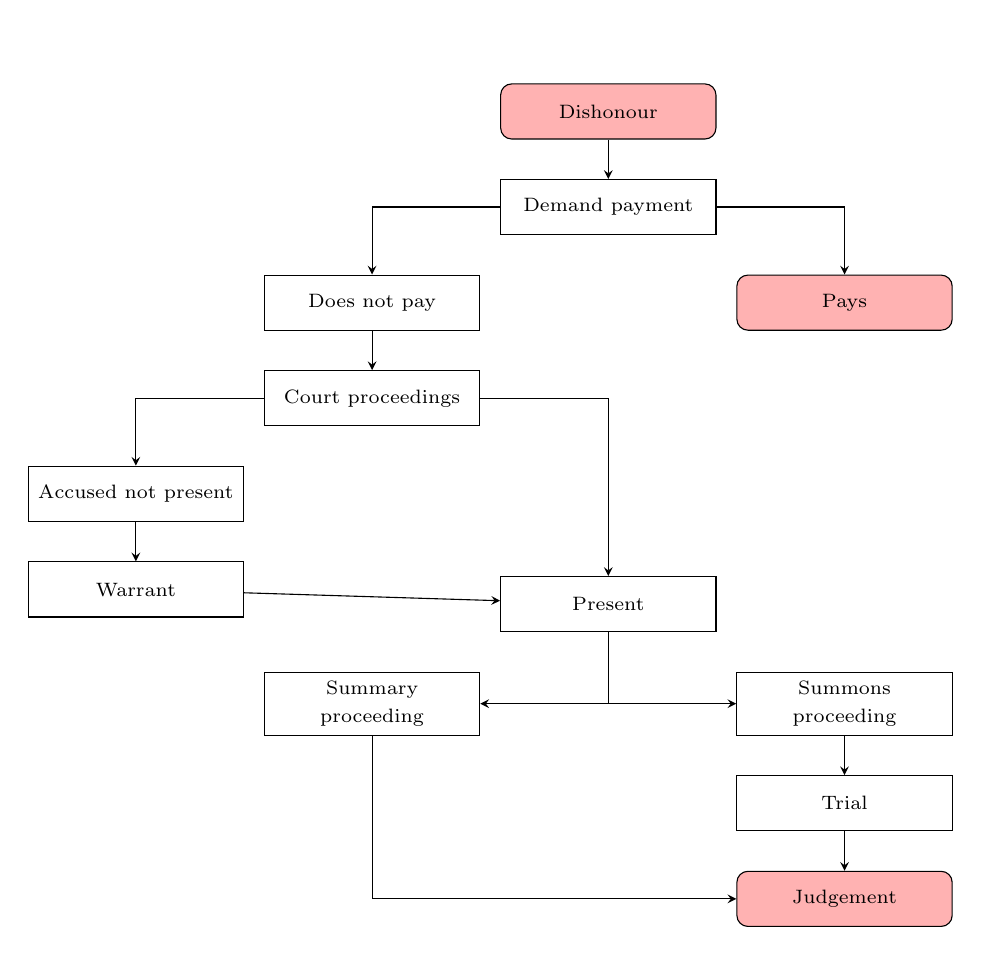
\begin{tikzpicture}[node distance= 1cm, text width=2.5cm]
\node (in0) [note] {};
\node (in1) [main, fill=red!30, below = 0.5cm of in0, yshift = 0.8cm] {Dishonour};
\node (in2) [process, below = 0.5cm of in1] {Demand payment};
\node (in3) [process, below = 0.5cm of in2, xshift = -3cm] {Does not pay};
\node (in4) [main, fill=red!30, below = 0.5cm of in2, xshift = 3cm] {Pays};
\node (in5) [process, below = 0.5cm of in3]{Court proceedings};
\node (in6) [process, below = 0.5cm of in5, xshift = -3cm] {Accused not present};
\node (in7) [process, below = 0.5cm of in6] {Warrant};
\node (in8) [process, below = 1.9cm of in5, xshift = 3cm] {Present};
\node (in9) [process, below = 0.5cm of in8, xshift = -3cm] {Summary proceeding};
\node (in10) [process, below = 0.5cm of in8, xshift = 3cm] {Summons proceeding};
\node (in11) [process, below = 0.5cm of in10] {Trial};
\node (in12) [main, fill=red!30, below = 0.5cm of in11] {Judgement};

\draw [arrow] (in1) -- (in2);
\draw [arrow] (in2) -| (in3);
\draw [arrow] (in2) -| (in4);
\draw [arrow] (in3) -- (in5);
\draw [arrow] (in5) -| (in6);
\draw [arrow] (in5) -| (in8);
\draw [arrow] (in6) -- (in7);
\draw [arrow] (in7) -- (in8);
\draw [arrow] (in8) |- (in9);
\draw [arrow] (in8) |- (in10);
\draw [arrow] (in10) -- (in11);
\draw [arrow] (in11) -- (in12);
\draw [arrow] (in9) |- (in12);

\end{tikzpicture}
\end{figure}

\pagebreak

\section{Robustness checks}
\label{sec:robustness}

\begin{landscape}
\pagestyle{empty}
\begin{table}
\centering
\caption{Disposal Days: Variation across States}\label{tab:durationStateWise}
\scalebox{0.75}{
\hspace*{-0.7cm}
\begin{tabular}{lcccccccccc}
\\[-1.8ex]
\hline \\[-1.8ex]
& \multicolumn{10}{c}{\textit{Dependent variable: Disposal days}} \\
\cline{2-11}
& (Punjab) & (Maharashtra) & (Karnataka) & (Himachal Pradesh) & (Haryana) & (Gujarat) & (Goa) & (Delhi) & (Chandigarh) & (Andhra Pradesh) \\
\hline \\[-1.8ex]
D(non-Appearance) & 282.470$^{***}$ & 117.295$^{***}$ & 219.113$^{***}$ & 217.113$^{***}$ & 231.698$^{***}$ & 193.737$^{***}$ & 261.782$^{***}$ & 227.051$^{***}$ & 329.881$^{***}$ & 152.268$^{***}$ \\
& (45.895) & (12.643) & (8.354) & (40.559) & (37.703) & (12.871) & (98.140) & (13.886) & (55.699) & (17.760) \\
& & & & & & & & & & \\
D(Summons) & 134.133$^{***}$ & 107.435$^{***}$ & 43.375$^{***}$ & 153.415$^{***}$ & 155.525$^{***}$ & 388.108$^{***}$ & 361.641$^{***}$ & $-$17.411 & 86.252$^{***}$ & 169.039$^{***}$ \\
& (10.040) & (19.458) & (11.362) & (40.332) & (11.272) & (26.752) & (59.235) & (14.558) & (20.949) & (21.555) \\
& & & & & & & & & & \\
D(Mediation) & 85.850$^{***}$ & 132.560$^{***}$ & 213.240$^{***}$ & 173.916$^{***}$ & 52.617$^{***}$ & 15.695 & 126.867$^{***}$ & $-$32.710$^{**}$ & 49.678$^{**}$ & 29.968 \\
& (10.097) & (13.157) & (10.996) & (36.869) & (11.094) & (20.682) & (48.674) & (15.447) & (22.164) & (27.086) \\
& & & & & & & & & & \\
D(Jurisdiction) & 203.741$^{***}$ & 320.802$^{***}$ & 263.146$^{***}$ & 238.843$^{***}$ & 223.542$^{***}$ & 347.000$^{***}$ & 221.767$^{**}$ & 253.748$^{***}$ & 172.153$^{***}$ & 202.846$^{***}$ \\
& (9.841) & (13.000) & (14.634) & (46.625) & (10.874) & (11.812) & (101.778) & (15.816) & (20.591) & (33.936) \\
& & & & & & & & & & \\
D(Multiplicity) & 146.651$^{***}$ & 293.331$^{***}$ & 230.515$^{***}$ & 99.971 & 93.660$^{***}$ & 18.436 & 162.484$^{*}$ & 101.022$^{***}$ & 156.640$^{***}$ & 160.606$^{***}$ \\
& (20.751) & (42.522) & (21.832) & (92.582) & (17.977) & (43.271) & (96.128) & (32.579) & (40.015) & (37.491) \\
& & & & & & & & & & \\
D(Contested) & 87.051$^{***}$ & $-$155.963$^{***}$ & $-$44.687$^{***}$ & $-$23.156 & 86.789$^{***}$ & $-$104.434$^{***}$ & $-$162.420$^{***}$ & $-$120.015$^{***}$ & 9.070 & $-$104.016$^{***}$ \\
& (17.045) & (15.169) & (8.636) & (52.987) & (16.530) & (17.941) & (54.347) & (21.355) & (31.604) & (20.176) \\
\hline \\[-1.8ex]
Year FE & Y & Y & Y & Y & Y & Y & Y & Y & Y & Y \\
\hline \\[-1.8ex]
Observations & 4,949 & 4,930 & 9,017 & 640 & 4,130 & 4,881 & 274 & 3,824 & 686 & 2,096 \\
R$^{2}$ & 0.214 & 0.245 & 0.246 & 0.259 & 0.209 & 0.301 & 0.260 & 0.259 & 0.251 & 0.149 \\
Adjusted R$^{2}$ & 0.213 & 0.243 & 0.245 & 0.248 & 0.207 & 0.300 & 0.232 & 0.257 & 0.240 & 0.145 \\
\hline \\[-1.8ex]
\multicolumn{11}{l}{\textit{Note:} $^{*}$p$<$0.1; $^{**}$p$<$0.05; $^{***}$p$<$0.01} \\
\end{tabular}}
\end{table}
\end{landscape}

\begin{landscape}
\pagestyle{empty}
\begin{table}
\centering
\caption{Number of hearings: Variation across States}\label{tab:hearingsStateWise}
\scalebox{0.75}{
\begin{tabular}{lcccccccccc}
\\[-1.8ex]
\hline \\[-1.8ex]
& \multicolumn{10}{c}{\textit{Dependent variable: Number of hearings}} \\
\cline{2-11}
& (Punjab) & (Maharashtra) & (Karnataka) & (Himachal Pradesh) & (Haryana) & (Gujarat) & (Goa) & (Delhi) & (Chandigarh) & (Andhra Pradesh) \\
\hline \\[-1.8ex]
D(non-Appearance) & 7.600$^{***}$ & 7.560$^{***}$ & 7.425$^{***}$ & 5.558$^{***}$ & 4.860$^{***}$ & 5.241$^{***}$ & 6.959$^{**}$ & 3.628$^{***}$ & 8.292$^{***}$ & 7.522$^{***}$ \\
& (1.329) & (0.329) & (0.220) & (0.654) & (0.966) & (0.339) & (2.955) & (0.174) & (1.501) & (0.628) \\
& & & & & & & & & & \\
D(Summons) & 5.428$^{***}$ & 8.064$^{***}$ & 7.352$^{***}$ & 4.930$^{***}$ & 5.504$^{***}$ & 17.208$^{***}$ & 14.333$^{***}$ & 1.858$^{***}$ & 4.982$^{***}$ & 18.646$^{***}$ \\
& (0.291) & (0.506) & (0.299) & (0.650) & (0.289) & (0.704) & (1.784) & (0.182) & (0.564) & (0.762) \\
& & & & & & & & & & \\
D(Mediation) & 3.415$^{***}$ & 3.068$^{***}$ & 6.631$^{***}$ & 3.598$^{***}$ & 2.316$^{***}$ & 0.452 & 5.820$^{***}$ & 0.955$^{***}$ & 1.678$^{***}$ & 2.993$^{***}$ \\
& (0.292) & (0.342) & (0.290) & (0.594) & (0.284) & (0.544) & (1.466) & (0.193) & (0.597) & (0.957) \\
& & & & & & & & & & \\
D(Jurisdiction) & 4.860$^{***}$ & 7.433$^{***}$ & 3.650$^{***}$ & 4.484$^{***}$ & 4.575$^{***}$ & 7.689$^{***}$ & 6.092$^{**}$ & 2.461$^{***}$ & 2.893$^{***}$ & 7.414$^{***}$ \\
& (0.285) & (0.338) & (0.386) & (0.751) & (0.279) & (0.311) & (3.065) & (0.198) & (0.555) & (1.199) \\
& & & & & & & & & & \\
D(Multiplicity) & 8.708$^{***}$ & 12.314$^{***}$ & 14.762$^{***}$ & 2.704$^{*}$ & 5.261$^{***}$ & $-$0.259 & 9.605$^{***}$ & 5.538$^{***}$ & 10.163$^{***}$ & 10.706$^{***}$ \\
& (0.601) & (1.106) & (0.575) & (1.492) & (0.460) & (1.139) & (2.895) & (0.407) & (1.078) & (1.325) \\
& & & & & & & & & & \\
D(Contested) & 10.062$^{***}$ & $-$1.049$^{***}$ & 1.758$^{***}$ & 2.959$^{***}$ & 8.682$^{***}$ & 0.513 & $-$0.066 & 0.466$^{*}$ & 4.183$^{***}$ & 0.958 \\
& (0.493) & (0.395) & (0.228) & (0.854) & (0.423) & (0.472) & (1.636) & (0.267) & (0.852) & (0.713) \\
\hline \\[-1.8ex]
Year FE & Y & Y & Y & Y & Y & Y & Y & Y & Y & Y \\
\hline \\[-1.8ex]
Observations & 4,949 & 4,930 & 9,017 & 640 & 4,130 & 4,881 & 274 & 3,824 & 686 & 2,096 \\
R$^{2}$ & 0.400 & 0.339 & 0.392 & 0.427 & 0.377 & 0.335 & 0.404 & 0.348 & 0.374 & 0.482 \\
Adjusted R$^{2}$ & 0.399 & 0.338 & 0.392 & 0.418 & 0.376 & 0.333 & 0.381 & 0.346 & 0.364 & 0.480 \\
\hline \\[-1.8ex]
\multicolumn{11}{l}{\textit{Note:} $^{*}$p$<$0.1; $^{**}$p$<$0.05; $^{***}$p$<$0.01} \\
\end{tabular} }
\end{table}
\end{landscape}

\newpage
\section{Survival model}
\label{sec:survivalModel}

Survival models have their origins in clinical research. The models estimate the probability of an event occurring within a specific time given that certain conditions are met. In our case, the model would estimate two things --- (1) the probability of a case remaining pending a certain number of years after filing, and (2) how different case characteristics affect the probability of the case concluding before the end date of observations (i.e., 15th September 2021).\footcite[For a prior example of the use of hazard models for empirical judicial analysis, see][]{datta2017_itatDelays}

Next, we estimate the effect of each case characteristic on the probability of the case getting disposed of by the observation period. Following \textcite{datta2017_itatDelays}, we use the Cox-proportional hazard model to estimate the effect of each case characteristic. Table \ref{tab:survialProb} shows the results of the Cox proportional hazard model. A negative coefficient indicates a lower probability of the case completing before the end of the observation period, and a positive coefficient indicates a higher probability of the case completing. As an example, jurisdictional issues and the non-appearance of the accused reduce the probability of the case concluding by approximately 51\%, whereas the case being contested increases this probability by 73\%.

The only result that contradicts the findings of the fixed-effects model is the effect of mediation on case duration. The results of the Cox-proportional hazard model indicate that being referred to mediation increases the probability of the case concluding within the observation period by 10.2\%. However, as we have mentioned earlier, we cannot reliably identify case characteristics in pending cases. Therefore, this result must be interpreted with some caution.

\newpage
{\footnotesize
\begin{longtable}[ht]{lr}
\caption{Regression result: Probability of case completion}\label{tab:survialProb}\\
\\[-1.8ex]
\hline \\[-1.8ex]
& \multicolumn{1}{c}{\textit{Dependent variable: Probability of case completion}} \\
\cline{2-2}
\hline \\[-1.8ex]

D(non-Appearance) & $-$0.712$^{***}$ \\
& (0.013) \\
D(Summons) & $-$0.286$^{***}$ \\
& (0.015) \\
D(Mediation) & 0.097$^{***}$ \\
& (0.013) \\
D(Jurisdiction) & $-$0.716$^{***}$ \\
& (0.013) \\
D(Multiple cheques) & $-$0.235$^{***}$ \\
& (0.027) \\
D(Contested) & 0.553$^{***}$ \\
& (0.015) \\
\hline \\[-1.8ex]
State & Y \\
Year & Y \\
\hline \\[-1.8ex]
Observations & 46,304 \\
R$^{2}$ & 0.274 \\
Max. Possible R$^{2}$ & 1.000 \\
Log Likelihood & $-$353,508.100 \\
Wald Test & 14,569.790$^{***}$ (df = 19) \\
LR Test & 14,819.270$^{***}$ (df = 19) \\
Score (Logrank) Test & 15,224.080$^{***}$ (df = 19) \\
\hline
\hline \\[-1.8ex]
\textit{Note:} & \multicolumn{1}{r}{$^{*}$p$<$0.1; $^{**}$p$<$0.05; $^{***}$p$<$0.01} \\
\end{longtable}}

\newpage
\section{Effect of 2015 amendment}
\label{sec:ni2015effect}

{\footnotesize \begin{longtable}{lcc|ccc}
\caption{Number of hearings: Variation across years}\label{tab:hearFE}
\\[-1.8ex]
\hline \\[-1.8ex]
& \multicolumn{5}{c}{\textit{Dependent variable: Number of hearings}} \\
\cline{2-6}
\\[-1.8ex] & 2014 & 2015 & 2016 & 2017 & 2018 \\
\hline \\[-1.8ex]
D(non-Appearance) & 5.996$^{***}$ & 6.809$^{***}$ & 6.929$^{***}$ & 7.764$^{***}$ & 8.049$^{***}$ \\
& (0.221) & (0.236) & (0.279) & (0.362) & (0.364) \\
& & & & & \\
D(Summons) & 3.773$^{***}$ & 5.041$^{***}$ & 7.678$^{***}$ & 10.391$^{***}$ & 11.416$^{***}$ \\
& (0.226) & (0.231) & (0.290) & (0.390) & (0.442) \\
& & & & & \\
D(Mediation) & 1.967$^{***}$ & 1.653$^{***}$ & 2.828$^{***}$ & 4.868$^{***}$ & 7.090$^{***}$ \\
& (0.213) & (0.220) & (0.267) & (0.375) & (0.446) \\
& & & & & \\
D(Jurisdiction) & 2.973$^{***}$ & 4.911$^{***}$ & 5.133$^{***}$ & 7.023$^{***}$ & 6.345$^{***}$ \\
& (0.244) & (0.235) & (0.262) & (0.350) & (0.352) \\
& & & & & \\
D(Multiplicity) & 5.756$^{***}$ & 8.732$^{***}$ & 9.122$^{***}$ & 10.539$^{***}$ & 12.298$^{***}$ \\
& (0.518) & (0.452) & (0.512) & (0.675) & (0.815) \\
& & & & & \\
D(Contested) & 5.157$^{***}$ & 4.213$^{***}$ & 3.139$^{***}$ & 2.230$^{***}$ & 1.341$^{***}$ \\
& (0.296) & (0.276) & (0.299) & (0.348) & (0.352) \\
\hline \\[-1.8ex]
State FE & Y & Y & Y & Y & Y \\
\hline \\[-1.8ex]
Observations & 6,760 & 8,458 & 8,165 & 6,117 & 5,927 \\
R$^{2}$ & 0.317 & 0.348 & 0.372 & 0.384 & 0.389 \\
Adjusted R$^{2}$ & 0.316 & 0.346 & 0.370 & 0.382 & 0.388 \\
\hline \\[-1.8ex]
\multicolumn{6}{l}{\textit{Note:} $^{*}$p$<$0.1; $^{**}$p$<$0.05; $^{***}$p$<$0.01} \\
\end{longtable}
}

\end{appendices}

\end{document}